\chapter{\label{ch:2-zvp}The Zero Vector Potential Absorption Mechanism}

\minitoc
\section{Motivations and an overview}
% TODO: \textbf{**This is from paper cover letter and acts as an abstract for this chapter, I also need to go through and add citations**}

Throughout the history of experimental science, light has always been the primary tool of investigation and discovery. Through the creation of synchrotron radiation sources and more recently XFELs, electron bunches have been employed to create increasingly specialised light sources for the study of matter of all kinds. At SLAC, the United States' forefront electron accelerator, applications hail from many disciplines: science, medicine, industry and homeland security. At Diamond Light Source, the UK's national synchrotron science facility, studies range from novel drugs to ancient paintings. Unsurprisingly, extensive research efforts have been enlisted to produce electron bunches of ever greater charge, energy and coherency. 
Multi-petawatt laser facilities are now available across the globe for the study of laser-plasma interactions in the ultra-relativistic regime $a_0 \gg 1$. Here, there is a novel method for high-charge electron bunch creation. Via relativistic effects, a laser pulse organises the electrons at the surface of a solid density plasma into coherent bunches that can be ejected at high speeds. Those discussed in this thesis have properties comparable to those of forefront accelerators but on ultra-short timescales. The quality, charge and duration of the attosecond electron bunches described here would enable the study of the most fundamental interactions of our universe. Electron bunch formation from solid targets has received much interest in recent years \cite{kulaginCharacteristicsRelativisticElectron2009, huEnhancedDenseAttosecond2015, cantonoExtensiveStudyElectron2018, serebryakovNearsurfaceElectronAcceleration2017, zhangGiantIsolatedAttosecond2020, hornyGenerationSingleAttosecond2021, ongElectronTransportNanowire2021, kulaginSubrelativisticInfraredTerahertz2021} with some experimental evidence for attosecond electron bunches from intense laser-solid interactions \cite{linIsolatedAttosecondElectron2020, cardenasSubcycleDynamicsRelativistic2019, thevenetVacuumLaserAcceleration2016}. This interest stems partially from their ability to produce higher charge bunches at lower intensities compared to gas targets \cite{linIsolatedAttosecondElectron2020}. Here is proposed a new mass-limited target setup to generate electron bunches of extreme charge density. These electron bunches are fully characterised in 3D \ac{PIC} simulations to compare their quality to those of existing electron bunch production methods. Their energies are described via an extended version of the \ac{ZVP} Mechanism and the corresponding implications for laser to plasma energy absorption are also considered including the intersection of \ac{ZVP} with \ac{SF-QED} effects of next generation laser facilities. \ac{ZVP} theory has direct relevance to \ac{HHG} due to the known intrinsic link between electron bunches and the reflection mechanism \cite{cousensElectronTrajectoriesAssociated2020, savinAttosecondscaleAbsorptionExtreme2017}.

These results have excited the community to perform experiments to realise these electron bunches for the creation of ultra-bright X-ray pulses: after the recent successful campaign at the ORION laser facility, studying \ac{HHG} from such electron bunches, details are presented here for the upcoming experiment to observe the electron bunches directly at the GEMINI PW laser at the Central Laser Facility, UK.

This Chapter is organised as follows. Section \ref{sec:zvp-intro} outlines the \ac{ZVP} mechanism including quantitative calculations of system properties. In Section \ref{sec:zvp-3Dsimulations} the first 3D PIC simulations to observe the ZVP mechanism are presented. Further PIC simulations are presented in Section \ref{sec:zvp-bunches} focusing now on the hot electron bunches produced via the mechanism their properties, energy scalings and implications for \ac{SF-QED}. Section \ref{sec:zvp-future_work} details the planned experiment to observe the ZVP mechanism at the GEMINI-PW laser facility including. Finally, concluding remarks are given in Section \ref{sec:zvp-conclusion}.

\section{Introduction}\label{sec:zvp-intro}
Of primary interest in this thesis is the interaction of a relativistically intense short-pulse laser interacting with a solid density plasma target with a sharp density gradient. Now is presented one model for the interaction: the \ac{ZVP} mechanism as proposed by \textit{Baeva et al} \cite{baevaZeroVectorPotential2011} and later developed by \textit{Savin et al} \cite{savinAttosecondscaleAbsorptionExtreme2017,savinModellingLaserPlasmaInteractions2019}. Alongside the theories of the Relativistic Electron Spring \cite{gonoskovUltrarelativisticNanoplasmonicsRoute2011, gonoskovUltrarelativisticNanoplasmonicsRoute2011} and Coherent Synchrotron Emission \cite{derbruggeEnhancedRelativisticHarmonics2010}, \ac{ZVP} is a post-ponderomotive model of attosecond absorption and reflection. The model considers a quasi-static surface equilibrium state analogously to ion acceleration in the hole boring \cite{vincentiOpticalPropertiesRelativistic2014} and light sail regimes \cite{macchiTheoryLightSail2014}.

% TODO: At some point I should briefly chat about other absorption models (I think at the end of the intro - this will also include the stuff above. - Then I will start this chapter by talking about the case where JxB does not apply. ALso in the intro specify that for an overdense plasma, the laser does not propagate and must be reflected and hence we are generally talking about a laser-plasma surface interaction and the implications thereof.) Before this point I also want to discuss preplasmas.

An explanation for the absorption of laser energy into dense plasmas was first suggested by Wilks and Kruer \cite{wilksAbsorptionUltraIntenseLaser1992}. A ponderomotive mechanism where plasma electrons are heated directly by the laser pulse via the $\mathbf{J}\times \mathbf{B}$ force. This thesis is interested in the so-called `post-ponderomotive' regime where the frequency of relativistic plasma oscillations ($\omega_\mathrm{p} \sim \sqrt{S}$) are greater than the $\mathbf{J}\times \mathbf{B}$ induced plasma electron oscillations at $2\omega_\mathrm{L}$. The plasma electrons' response is then fast enough to compensate the ponderomotive pressure of the laser pulse with the formation of electrostatic fields between electrons and ions and so respond adiabatically to the applied $\mathbf{J}\times \mathbf{B}$ force. Hence, plasma electrons cannot be heated directly by the laser pulse. Interestingly, this condition suggests a criterion for the \ac{ZVP} regime, $S > 4$, slightly more constraining than $S>1$ as is typically stated for the \ac{ZVP} regime \cite{savinModellingLaserPlasmaInteractions2019}. The bulk plasma must have $S>1$ to prevent relativistic transparency and so ensure a laser-surface interaction. Then the ponderomotive pressure of the laser will typically compress the front surface to densities such that the overdensity condition is satisfied, provided the target is of sufficient thickness. Note that to neglect the pre-adiabatic formation phase requires a sufficiently steep density gradient around the relativistic critical density surface (where $S=1$) to shift the main interaction to a region where this condition on the overdensity is satisfied. Pre-plasma formation and scale length will be discussed in great detail in the following chapters. For now, assume the technology exists to control this phenomenon. 

Provided all conditions are met, the ponderomotive pressure of the laser pulse compresses electrons at the front surface of the plasma and so shifts the laser-plasma surface interaction to plasma densities well beyond the relativistic critical density, leaving in its wake a positive space charge of ions. This electron-ion charge separation leads to the formation of a \textit{pseudo-capacitor} electrostatic field. Having entered a regime of adiabaticity, the plasma skin layer is confined within a potential well consisting of the ponderomotive pressure of the laser pulse and the Coulomb potential of the pseudocapacitor field. Thus is formed a high density and longitudinally thin electron bunch (sometimes referred to as an electron sheath in the literature \cite{gonoskovUltrarelativisticNanoplasmonicsRoute2011}) at the plasma surface.

To understand this system, consider now a relativistic linearly polarised laser pulse obliquely incident, at an angle of incidence $\theta$, on a semi-infinite plasma, existing for $x\ge0$ as in figure \ref{fig:zvpforcesppol}.

\begin{figure}
	\centering
	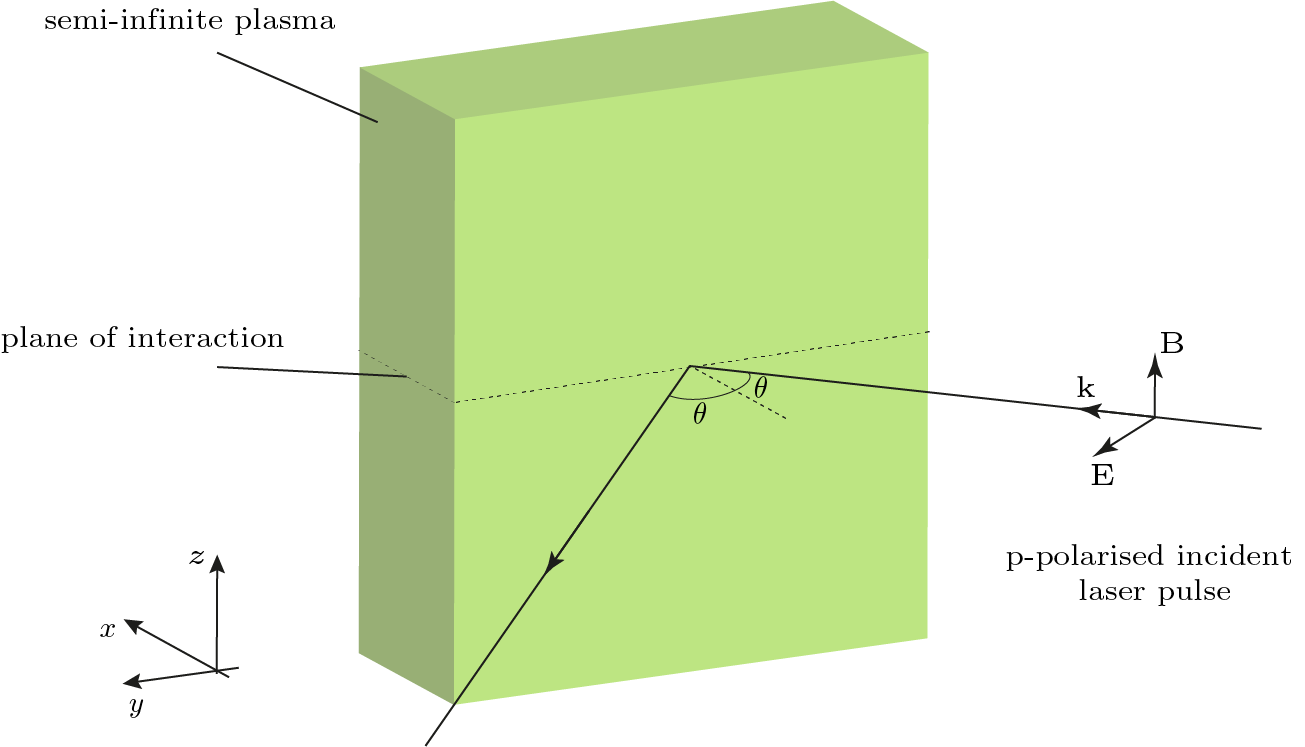
\includegraphics[width=0.7\linewidth]{figures/zvp/zvp_forces_ppol}
	\caption[Diagram of a p-polarised laser pulse incident at angle $\theta$ specularly reflected from a solid density plasma.]{Diagram of a p-polarised laser pulse incident at angle $\theta$ specularly reflected from a solid density plasma. By considering the Lorentz force equation, it is clear that all forces and therefore all plasma particle dynamics are confined to a plane.}
	\label{fig:zvpforcesppol}
\end{figure}
The Hamiltonian of a single electron confined within the potential well \cite{goldsteinClassicalMechanics2013} is
\begin{equation}\label{eq:hamiltonian_general}
	\mathcal{H} = c\sqrt{m^2_\mathrm{e}c^2 + |\mathbf{p}|^2} - e\Phi.
\end{equation}
Here, the second term of equation \ref{eq:hamiltonian_general} describes the contribution to the electron's energy from the electrostatic potential, $\Phi$, of the pseudo-capacitor. The first term is the electron energy, $U$, extracted from the invariant of the relativistic 4-momentum of the electron, $\mathbf{P^\mu} = (U/c, \mathbf{p})$,
\begin{equation}\label{eq:zvp-energy_invariant}
	\mathbf{P_\mu  P^\mu} = \frac{U^2}{c^2} - |\mathbf{p}|^2 = m^2_\mathrm{e}c^2.
\end{equation}

Decomposing the electron's 3-momentum into orthogonal components: $p_\mathrm{prop}$, along the laser propagation direction, $p_\mathrm{pol}$, along the polarisation axis of the laser pulse and $p_\perp$, perpendicular to both, there are two simplifications to be made. Firstly, by canonical conservation of transverse momentum, $p_\mathrm{pol} = eA$, where $A$ is the laser vector potential amplitude. Secondly, in the case of a p-polarised laser pulse (the known optimum for ZVP electron bunch generation \cite{savinAttosecondscaleAbsorptionExtreme2017} and \ac{HHG} \cite{baevaTheoryHighorderHarmonic2006}), with reference to figure \ref{fig:zvpforcesppol} and the Lorentz force law, the forces at play confine the electron trajectory to the $p_\mathrm{prop}$-$p_\mathrm{pol}$ plane and the essential interaction geometry is two-dimensional. This is provided one considers length scales smaller than the focal spot of the laser pulse on the target, such that variation of the ponderomotive pressure with the third dimension can be neglected.

Explicitly, the Hamiltonian can be written as
\begin{equation}\label{eq:hamiltonian_specific}
	\mathcal{H} = c\sqrt{m^2_ec^2 + p^2_\mathrm{prop} + e^2A^2} - e\Phi.
\end{equation}
From equation \ref{eq:hamiltonian_specific} it is clear that should the vector potential pass through zero, one of potential well walls is totally suppressed, enabling electrons in the skin layer to escape the plasma, breaking adiabaticity. The necessity of vector potential zeros for this violent reconstruction of the plasma surface led Baeva \textit{et al} \cite{baevaZeroVectorPotential2011} to coin the term `Zero Vector Potential' mechanism to describe this process. Indeed, while elementary electromagnetism tells us a laser pulse will exponentially decay within a skin layer of a plasma without passing through zero, Baeva \textit{et al} \cite{baevaZeroVectorPotential2011} demonstrated in \ac{PIC} simulations that in this non-linear regime, zeros do exist and do propagate through the skin layer. The explanation relies on a Doppler shift in the laser field due to the relativistic motion of the ablating plasma surface, and a mathematical formalism of this process proceeds as follows.

% TODO: \textbf{**Must also discuss the impact of relativity in creating the observed phenomena, probably at energy scaling section?**}

As the \ac{ZVP} mechanism is a relativistic phenomenon, it is absolutely essential to perform a relativistic analysis. Since all accelerated electrons travel at approximately speed $c$, surface electrons undergo similar trajectories. Acting collectively they oscillate in the laser pulse field. Consider first a transformation to the frame of reference where the laser pulse is normally incident to the plasma surface, this frame travels at velocity $\mathbf{v} = (c\sin\theta )\hat{\mathbf{y}}$ with electrons streaming at $-\mathbf{v}$. 
Using equation \ref{eq:zvp-energy_invariant}, $U = \gamma m_\mathrm{e} c^2$ and integrating equation \ref{eq:intro-transverse_momentum_differential_equation} in the boosted frame noting $p_\mathrm{T}(t=0) = \gamma_\mathbf{v} m_\mathrm{e}v =m_\mathrm{e}c \sin\theta\cos\theta$,
\begin{equation}
	\gamma^2 = 1 + (a_0 + \sin\theta\cos\theta)^2 + \left(\frac{p_\mathrm{prop}}{m_\mathrm{e}c}\right)^2,
\end{equation}
where all parameters are in the boosted frame. Using $\mathbf{p} = \gamma m_\mathrm{e} \mathbf{v}$, the longitudinal velocity is
\begin{equation}
	v_\mathrm{prop} = \frac{\tilde{p}_\mathrm{prop}c}{\sqrt{1 + (a_0 + \sin\theta\cos\theta)^2 + \tilde{p}^2_\mathrm{prop}}},
\end{equation}
where $\tilde{p}_\mathrm{prop} = p_\mathrm{prop}/m_\mathrm{e}c$. Thus, should the transverse vector potential pass through $-\sin\theta\cos\theta$, zero for normal incidence, the surface can propagate towards the laser pulse at very close to speed $c$. Transforming back to the laboratory frame, at the peak of ablation ($\mathbf{u}\approx -c\hat{\mathbf{x}}$) and using the equations for relativistic velocity addition,
\begin{equation}\label{eq:zvp_velocityaddition1}
	\mathbf{u}'_{\|} = \frac{\mathbf{u}-\mathbf{v}}{1- \mathbf{u}\cdot\mathbf{v}/c^2},
\end{equation}
\begin{equation}\label{eq:zvp_velocityaddition2}
	\mathbf{u}'_{\perp} = \frac{\mathbf{u}_\perp}{\gamma_v(1- \mathbf{u}\cdot\mathbf{v}/c^2)},
\end{equation}
where $\gamma_v = 1/\sqrt{1-|\mathbf{v}|^2/c^2}$ \cite{steaneRelativityMadeRelatively2012}, one finds that this peak ablation at speed $\approx c$ occurs now in the specular reflection direction. Simultaneity is broken and ripples co-move along the surface with the incident laser pulse wavefronts.

Transform now to the rest frame of the ablating front. Beyond the relativistic critical density surface, the vector potential of the laser pulse decays evanescently. At the spatial centre of the laser pulse, it can be described simply by
\begin{equation}
	\mathbf{A}'_\mathrm{L}(t',r') = A'_0\cos(\omega'_\mathrm{L}t')\exp(-r'/\delta')\hat{\mathbf{r}}'_\mathrm{pol}= A'_\mathrm{L}\hat{\mathbf{r}}'_\mathrm{pol},
\end{equation}
where the primed symbols indicate that these quantities are measured in the rest frame of the expanding front. $A'_0$ is the vector potential amplitude and $\omega'_\mathrm{L}$ is the frequency of the laser pulse, $r'$ is the propagation distance of the laser into the plasma, $\delta'$ is the skin depth and $\hat{\mathbf{r}}'_\mathrm{pol}$ a unit vector defining the polarisation direction of the laser pulse. Un-primed coordinates will indicate the lab frame measurements.

% TODO PIC simulation of surface ripples?

While previous demonstrations of the existance of vector potential zeros assumed that the ablation occurs normal to plasma surface, it is necessary to confirm that zeros are still predicted for specular ablation. Consider a p-polarised laser pulse confined to the $x$-$y$ plane incident with an angle of incidence $\theta$ on an ablating overdense plasma expanding with velocity $-v_f\hat{\mathbf{x}}$ in the lab frame, as in figure \ref{fig:zvp_ablatingfront}.

\begin{figure}
	\centering
	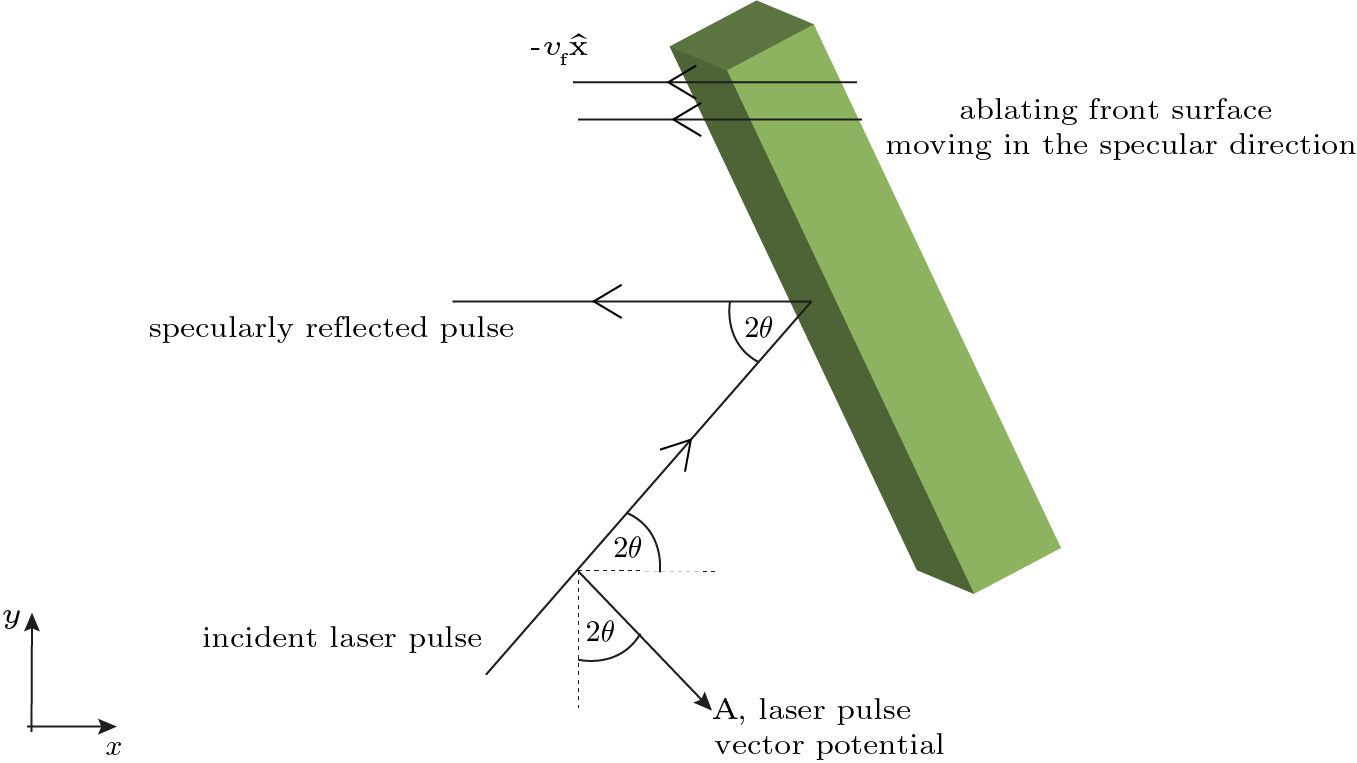
\includegraphics[width=0.7\linewidth]{figures/zvp/zvp_ablating_front}
	\caption[Diagram of a $p$-polarised laser pulse incident on an ablating overdense plasma.]{Diagram of a $p$-polarised laser pulse incident on an ablating overdense plasma. The laser is incident obliquely at an angle of $\theta$ and is reflected specularly. The plasma ablates specularly also. The interaction geometry is confined to a 2D plane.}
	\label{fig:zvp_ablatingfront}
\end{figure}
The direction of polarisation is
\begin{equation}
	\hat{\mathbf{r}}_\mathrm{pol} = \hat{\mathbf{x}}\sin{2\theta} - \hat{\mathbf{y}}\cos{2\theta}
\end{equation}
and the velocity of the rest frame of the ablating front relative to the lab frame is $-v_f\hat{\mathbf{x}}$.

Applying the Lorentz transformation to the electromagnetic 4-potential, $\mathbf{A}^\mu$, where $\Lambda_\mu^\nu$ is given by equation \ref{eq:zvp_lorentz}, immediately from the $y$-coordinate transformation,
\begin{equation}\label{eq:zvp_lorentz_y}
	A'_\mathrm{L}\cos{2\theta'} = A_\mathrm{L}\cos{2\theta}.
\end{equation}
Applying the headlight effect for a source moving at an angle $2\theta$ to the boosted frame (a full derivation is given in Appendix \ref{sec:app_headlight}),
\begin{equation}
	\cos{(2\theta')} = \frac{\cos{(2\theta)}-\beta}{1 - \beta\cos{(2\theta)}}
\end{equation}
and rearranging equation \ref{eq:zvp_lorentz_y}, the vector potential in the lab frame is
\begin{equation}\label{eq:zvp_labA}
	A_\mathrm{L} = \frac{1-\beta \sec{(2\theta)}}{1 - \beta\cos{(2\theta)}} A'_0\cos{(\omega'_L t')}\exp{(-r'/\delta')}.
\end{equation}
Writing the boosted frame space-time coordinates in terms of the lab frame coordinates,
\begin{equation}
	ct' = \gamma(ct-\beta x),
\end{equation}
\begin{equation}
	x' = \gamma(x-\beta ct),
\end{equation}
yields
\begin{equation}\label{eq:zvp_labAfull}
	A_\mathrm{L} =  A_0\cos{(\omega_L t - kx)}\exp{\left(-\frac{\sqrt{(x-\beta ct)^2+(y/\gamma)^2}}{\delta}\right)},
\end{equation}
where
\begin{equation}
	A_0 = \frac{1-\beta \sec{(2\theta)}}{1 - \beta\cos{(2\theta)}}A'_0,
\end{equation}
\begin{equation}
	\omega_L = \gamma \omega'_L,
\end{equation}
\begin{equation}
	k = \frac{\beta \gamma\omega'_L}{c},
\end{equation}
\begin{equation}
	\delta = \frac{\delta'}{\gamma}.
\end{equation}
The oscillatory term in equation \ref{eq:zvp_labAfull} demonstrates the propagation of vector potential zeros within the plasma target. From the structure of this term it would appear that these zeros are expelled from the plasma along the specular direction at a speed
\begin{equation}\label{eq:zvp-zero_v}
	v_\phi = \frac{\omega_L}{k} = \frac{c}{\beta} = -\frac{c^2}{v_\mathrm{f}}.
\end{equation}
While in their original ZVP paper Baeva laid some doubt on their version of this calculation, instead suggesting similarity theory predicts zeroes propagate at speed $c$ \cite{baevaZeroVectorPotential2011}, the theory of High Harmonic Generation rejects this alternative. It is well known that the emission of reflected radiation occurs primarily at the point where the transverse vector potential passes through zero \cite{cousensElectronTrajectoriesAssociated2020} but equally that the width of the radiated pulse depends on the advance time emission point \cite{edwardsXRayEmissionEffectiveness2020}. If the zeroes moved at speed $c$, then the observed emitted pulse would be infinitely thin, producing radiation with perfect coherence in all cases. In practice however, simulations have suggested advanced time bunch widths are finite and decreasing with increasing laser intensity \cite{edwardsXRayEmissionEffectiveness2020}. This is precisely what is predicted by equation \ref{eq:zvp-zero_v}. As the laser intensity increases, $v_\mathrm{f}$ naturally increases and thus the zeroes propagate closer to the speed of light, reducing the advanced time bunch width.

After expulsion from the plasma alongside zeroes of the vector potential they release CSE, then they accelerate and they they are rotated back.


To summarise, for a sufficiently intense laser pulse, electrons at the surface of an irradiated solid target are accelerated by the laser to relativistic velocities at a fraction of a laser pulse cycle and therefore electrons both follow similar trajectories and respond adiabatically to the $\mathbf{J}\times \mathbf{B}$ force of the laser pulse. They form into a high charge density spatially thin coherent electron bunch on the front surface of the plasma but displaced inwards from the approximately immobile ions via the ponderomotive pressure of the laser. This charge separation generates a longitudinal electrostatic pseudocapacitor field that confines electrons to a potential well on the front surface of the plasma, preventing further propagation of the electron bunch into the plasma bulk. When the zero of the vector potential passes through the electron bunch, the ponderomotive pressure instantaneously vanishes and electrons are ejected specularly from the target, co-propagating with the zeroes of the vector potential and gaining energy as they discharge the pseudocapacitor field. The electron bunch is then rotated by the laser pulse and launched into the bulk at high energy, as it does so emitting coherent synchrotron radiation in transmission and reflection.

\subsection{ZVP electron bunch energies}\label{sec:zvp_energies_derivation}
In \cite{baevaZeroVectorPotential2011}, Baeva \textit{et al} propose energy scalings for electron bunches produced in the \ac{ZVP} regime as a function of the incident laser pulse intensity and plasma density. Later this was then extended to \ac{3D} by Savin \textit{et al} \cite{savinAttosecondscaleAbsorptionExtreme2017}. What follows is that discussion with closer consideration of both the constants of proportionality and their consequences. Note that throughout the electron bunch is treated as infinitessimally thin, as proved to be a reasonable assumption in previous work on ZVP \cite{baevaTheoryHighorderHarmonic2006, savinAttosecondscaleAbsorptionExtreme2017, savinEnergyAbsorptionLaserQED2019}. Sub-bunch dynamics have been explored in more detail by Gonoskov \textit{et al} \cite{gonoskovTheoryRelativisticRadiation2018}.

Consider again the semi-infinite block of plasma presented in figure \ref{fig:introplasmafrequency}, normally irradiated by a laser pulse with wavelength $\lambda_\mathrm{L}$ and peak electric field, $E_\mathrm{L}$. It is now the ponderomotive pressure of the laser that displaces the electron fluid. The electron surface moves inwards until the pressure exerted by the peak instantaneous ponderomotive pressure of the laser pulse cycle,
\begin{equation}
	\mathbf{P}_\mathrm{L} = \epsilon_0 E^2_\mathrm{L} \hat{\mathbf{x}} = \epsilon_0 \left(\frac{a_0\omega_\mathrm{L}m_\mathrm{e}c}{e}\right)^2 \hat{\mathbf{x}}
\end{equation}
is equal and opposite to the pressure exerted by the pseudo-capacitor field,
\begin{equation}
	\mathbf{P}_\mathrm{C} = \frac{QE_\mathrm{C}}{\sigma} \hat{\mathbf{x}}= -\frac{(en_\mathrm{e}\Delta x)^2}{\epsilon_0}\hat{\mathbf{x}}
\end{equation} 
from equations \ref{eq:intro_Q} and \ref{eq:intro_E}. Equating the magnitudes of $\mathbf{P}_\mathrm{L}$ and $\mathbf{P}_\mathrm{C}$, the maximum displacement inwards of electrons is
\begin{equation}\label{eq:zvp_dx}
	\Delta x \hat{\mathbf{x}} = \frac{c}{\omega_\mathrm{L}}\frac{a_0}{\bar{n}_\mathrm{e}}\hat{\mathbf{x}}  = \frac{1}{kS}\hat{\mathbf{x}},
\end{equation}
where $k$ is the wave-vector of the laser pulse. Correspondingly,
\begin{equation}\label{eq:zvp_E}
	E_\mathrm{C} = \frac{en_\mathrm{e}}{\epsilon_0}\Delta x = \frac{\omega_\mathrm{L}cm_\mathrm{e}a_0}{e} = E_\mathrm{L}.
\end{equation}
Applying the results of equations \ref{eq:zvp_dx} and \ref{eq:zvp_E}, when the ponderomotive pressure vanishes and the electron bunch is launched across the pseudo-capacitor, the relativistic kinetic energy gained by a single electron is
\begin{equation}\label{eq:zvp_T}
	T =  \int \mathbf{F}\cdot\mathrm{d}\mathbf{s} = \int^0_{\Delta x} -eE_\mathrm{C}dx = \int^0_{\Delta x}-\frac{en_\mathrm{e}x}{\epsilon_0}dx = \frac{1}{2}m_\mathrm{e}c^2\frac{a^2_0}{\bar{n}_\mathrm{e}}
\end{equation}
or an electron gamma factor,
\begin{equation}\label{eq:zvp_gamma}
	\gamma = \frac{1}{\sqrt{1-\beta^2}} = 1 + \frac{a_0^2}{2\bar{n}_\mathrm{e}}.
\end{equation}
Assuming all displaced electrons are captured by the potential well and launched as a coherent bunch, the total number of electrons in the bunch is
\begin{equation}\label{eq:zvp-Ne}
	N_\mathrm{e} = n_\mathrm{e} \sigma \Delta x = \frac{\sigma a_0 n_\mathrm{c}}{k}  = \sigma \epsilon_0 E_\mathrm{L}
\end{equation}
and hence, the total kinetic energy of the electron bunch is
\begin{equation}\label{eq:zvp_U}
	U_\mathrm{ZVP} = N_\mathrm{e} T = \frac{\sigma n_\mathrm{c}}{k}\times \frac{1}{2}m_\mathrm{e}c^2 \frac{a^3_0}{\bar{n}_\mathrm{e}}.
\end{equation}
It is now interesting to compare equation \ref{eq:zvp_U} to the laser energy deposited upon the plasma surface and therefore consider what fraction of the laser energy can be absorbed via the \ac{ZVP} mechanism. Using $E_\mathrm{C} = E_\mathrm{L}$, equation \ref{eq:zvp_U} can be rewritten as
\begin{equation}
	U_\mathrm{ZVP} = \frac{1}{2\omega_\mathrm{L} S}\sigma c \epsilon_0 E^2_\mathrm{L}.
\end{equation}
For the case of normal incidence, bunches are produced at a frequency of $2\omega_\mathrm{L}$, naturally following the frequency of the $\mathbf{J}\times \mathbf{B}$ force. Assuming a sinusoidal plane wave incident with surface area $\sigma$, the energy available during the pushing phase (a quarter-cycle) is
\begin{equation}
	 U_\mathrm{L,1/4} = \sigma \frac{T}{4}\langle I_\mathrm{L}\rangle = \frac{2\pi}{8\omega_\mathrm{L}}\sigma c\epsilon_0E^2_\mathrm{L}.
\end{equation}
Hence,
\begin{equation}
	\eta_\mathrm{ZVP} = \frac{U_\mathrm{ZVP}}{U_\mathrm{L,1/4}} = \frac{2}{\pi S}.
\end{equation}
Interestingly, this analytical result predicts the trend observed by A. Savin \cite{savinModellingLaserPlasmaInteractions2019} in \ac{PIC} simulations both in magnitude and in scaling. Indeed, A. Savin demonstrated 
\begin{equation}
	\eta_\mathrm{ZVP} \sim S^{-1.000(3)},
\end{equation}
however, this result led A. Savin to conclude that increasing $S$ reduces absorption, increasing the energy in the reflected \ac{HHG} beam thus increasing high harmonic efficiency, seemingly in tension with the results of other works \cite{gonoskovUltrarelativisticNanoplasmonicsRoute2011,edwardsXRayEmissionEffectiveness2020}. The resolution arises from awareness of two distinct conversion efficiencies that describe the reflected harmonic spectrum: the total conversion efficiency into the full reflected beam and the conversion efficiency for individual harmonics. While the total conversion into the reflected beam decreases for decreasing $S$, the slope of the harmonic spectrum also decreases, reducing \ac{HHG} efficiency. Indeed, high X-ray harmonic efficiency necessitates high reflection inefficiencies due to the production of ZVP electron bunches as higher energy bunches produce more coherent reflected radiation \cite{edwardsXRayEmissionEffectiveness2020}, a caveat not often considered in the quest for higher-order harmonics. The impact of the ZVP mechanism on \ac{HHG} will be discussed in great detail in the following chapter.

The expressions for energies in equations \ref{eq:zvp_T} and \ref{eq:zvp_U} require the electron bunch to fully discharge the pseudo-capacitor before interaction with the subsequent laser pulse peak. Since the electron bunch travels at speed $\approx c$, the peak displacement (and thus the pseudo-capacitor width) must satisfy
\begin{equation}\label{eq:zvp-deltax_condition}
	\Delta x \le \frac{\lambda}{8}.
\end{equation}
Using equation \ref{eq:zvp_dx}, it is clear equation \ref{eq:zvp-deltax_condition} is satisfied for $ S\ge 1.3$ for normal incidence.

\subsection{ZVP bunches oblique incidence scaling and internal bunch structure}
This section is inspired by ideas from the work of Gonoskov \textit{et al} \cite{gonoskovUltrarelativisticNanoplasmonicsRoute2011} and Vincenti \textit{et al} \cite{vincentiOpticalPropertiesRelativistic2014} to extend the theory of the ZVP mechanism for energy absorption to the more practical\footnote{Not only is this more feasible in experiment but has been shown to optimise HHG \cite{gonoskovUltrarelativisticNanoplasmonicsRoute2011}.} case of oblique incidence. 

Provided the plasma-vacuum boundary is sufficiently steep, the plasma electrons will respond adiabatically to the laser pulse and arrange themselves to form a pseudocapacitor longitudinal electric field $E_\mathrm{C}$ at the plasma surface. At all points in this adiabatic `pushing' phase, the surface electrons will be in a quasi-static equilibrium \textit{i.e.} there will be a balance between the electromagnetic forces on them. Consider again the laser pulse incident on a solid density plasma existing for $x>0$ at angle $\theta$. Transforming to the frame of reference in which the laser is normally incident (quantities in this frame are indicated by the primed symbol), the electron and ion bulk plasma species stream at velocity $\mathbf{v}_\mathrm{d} = -c \sin\theta \hat{\mathbf{y}}$.  Applying the Lorentz force law along the longitudinal direction ($\hat{\mathbf{x}}$), for a displacement of the electron fluid $x'_\mathrm{e}$ (one assumes that the expression for a single electron at the surface describes the surface since all electrons follow similar trajectories), travelling at speed $\mathbf{v'}$,
\begin{equation}\label{eq:zvp_eq}
	-e(\mathbf{v'}(x'_\mathrm{e})\times (\mathbf{B}'_\mathrm{L}(x'_\mathrm{e}) + \mathbf{B}'_\mathrm{i}(x'_\mathrm{e}))\cdot \hat{\mathbf{x}} + E'_\mathrm{C}(x'_\mathrm{e}) )= 0,
\end{equation}
where the laser magnetic field,
\begin{equation}\label{eq:zvp_Bl}
	B'_\mathrm{L} = \frac{m_\mathrm{e} \omega'_\mathrm{L}a_0\sin(\omega'_\mathrm{L}t'-k'x'_\mathrm{e})}{e} \hat{\mathbf{z}}
\end{equation}
and $B_\mathrm{i}$ is the magnetic field generated by the uncompensated ion current, $\mathbf{J_\mathrm{i}} =  Zen'_\mathrm{i}(x'_\mathrm{e}) \mathbf{v}_\mathrm{d}$, where the electron fluid has been displaced. As before, from equation \ref{eq:intro_E},
\begin{equation}\label{eq:zvp_Ec}
	E'_\mathrm{C} = \frac{en'_\mathrm{e}x'_\mathrm{e}}{\epsilon_0}.
\end{equation}
Applying Maxwell-Ampère's Law, equation \ref{eq:intro-B1}, and noting that by symmetry there can be no variation in the magnetic field with $y'$ or $z'$, it becomes clear that
\begin{equation}\label{eq:zvp_BiJi}
	-\frac{\mathrm{d}(\mathbf{B}'_\mathrm{i})_{z'}}{\mathrm{d} x'} = \mu_0 (\mathbf{J}_\mathrm{i})_{y'}.
\end{equation}
Integrating equation \ref{eq:zvp_BiJi} from $-\infty$ to $x'_\mathrm{e}$, noting that $\mathbf{B}_\mathrm{i} = 0$ at infinity and assuming a constant density profile $n'_\mathrm{i}$ for $x>0$ with $Zn_\mathrm{i} = n_\mathrm{e}$,
\begin{equation}\label{eq:zvp_Bi}
	\mathbf{B}'_\mathrm{i}(x'_\mathrm{e}) = \mu_0 en'_\mathrm{e}x'_\mathrm{e}c\sin(\theta)\hat{\mathbf{z}}.
\end{equation}
Using equations \ref{eq:zvp_Bl}, \ref{eq:zvp_Ec} and \ref{eq:zvp_Bi} and making the reasonable approximation that the relativistic electrons on the surface move at speed $v'_y \approx \pm c$ at peak displacement ($x'_\mathrm{e} = x'_\mathrm{p}$), \ref{eq:zvp_eq} can be written as
\begin{equation}
	-e\left(\pm c\left(\pm\frac{m_\mathrm{e}\omega'_\mathrm{L}a_0}{e} + \mu_0 en'_\mathrm{e} x'_\mathrm{p}c\sin\theta\right)+\frac{en'_\mathrm{e}x'_\mathrm{p}}{\epsilon_0}\right) = 0.
\end{equation}
For the laser to be in the pushing phase, the first term must be negative, corresponding to $\mathbf{v'}$ and $\mathbf{B}'_\mathrm{L}$ having the opposite sign, hence,
\begin{equation}
	 c\left(-\frac{m_\mathrm{e}\omega'_\mathrm{L}a_0}{e} \pm \mu_0 en'_\mathrm{e} x'_\mathrm{p}c\sin\theta\right)+\frac{en'_\mathrm{e}x'_\mathrm{p}}{\epsilon_0} = 0,
\end{equation}
where here the $\pm$ tracks the sign of $\mathbf{v}'$. After some maniputation, one arrives at
\begin{equation}
	x'_\mathrm{p} = \frac{1}{k'S' (1\pm \sin\theta)}.
\end{equation}
Transforming back to the lab frame,
\begin{equation}
	x_\mathrm{p} = \frac{\cos^2\theta}{kS(1\pm \sin\theta)}.
\end{equation}
Convincingly this reduces to equation \ref{eq:zvp_dx} for $\theta =0$ and predicts the suppression and enhancement of the two surface oscillations per laser pulse cycle. Explicitly, for a laser pulse propagating at $y = x\tan\theta$, the peak displacement of the electron surface is enhanced for $\mathbf{B}_\mathrm{L}$ in the $+\hat{\mathbf{z}}$-direction and suppressed for $\mathbf{B}_\mathrm{L}$ in the $-\hat{\mathbf{z}}$-direction.

Again, integrating to find the work done as the electron bunch accelerates across the pseudocapacitor,
\begin{equation}\label{eq:zvp_Tzvp_theta}
	T (\theta)=  \int \mathbf{F}\cdot\mathrm{d}\mathbf{s} = \frac{1}{2}m_\mathrm{e}c^2\frac{a^2_0}{\bar{n}_\mathrm{e}}\frac{\cos^4\theta}{(1\pm \sin\theta)^2}.
\end{equation}
While it was to be expected that a component of the electric field acting into or out of the plasma would change the magnitude of the displacement, this result suggests that increasing the angle of incidence can increase the electron energy gain in the enhanced cycle more than the decrease in the suppressed cycle. Note that this is to be expected as it is known that HHG efficiency is improved for non-zero angle of incidence \cite{gonoskovUltrarelativisticNanoplasmonicsRoute2011, edwardsXRayEmissionEffectiveness2020}. It would be interesting to explore whether the presence of an external magnetic field could be applied to mimic the effect of oblique incidence by replacing the magnetic field due to the uncompensated ion current.

While this model would suggest an optimal angle for electron energy and therefore of \ac{HHG} of $\pi/2$, if $\theta > \pi/4$, then, if the relativistic electron bunch is travelling at $c$ along the specular reflection direction, the subsequent laser peak amplitude will never `catch up' with the electron bunch, and electrons can escape, generating high charge electron bunches in reflection as observed in experiment by Lin \textit{et al }\cite{linIsolatedAttosecondElectron2020}, but reducing the efficiency of HHG.

Finally, the total bunch energy as a function of $\theta$,
\begin{equation}\label{eq:zvp_Uzvp_theta}
	U_\mathrm{ZVP}(\theta) = \frac{\sigma n_\mathrm{c}}{k}\times \frac{1}{2}m_\mathrm{e}c^2 \frac{a^3_0}{\bar{n}_\mathrm{e}}\frac{\cos^6\theta}{(1\pm \sin\theta)^3}.
\end{equation}
Thus oblique incidence can increase laser absorption efficiency for higher $S$ plasmas which are currently more easily accessed compared to the more optimal low $S$ plasmas.

\subsection{Defining characteristics of the ZVP mechanism}\label{sec:zvp-characteristics}
In her original paper on the ZVP mechanism, T. Baeva \textit{et al} \cite{baevaZeroVectorPotential2011} outlined 6 defining characteristics of the \ac{ZVP} mechanism, namely,
\begin{enumerate}
	\item The existence of vector potential zeros moving through the skin layer in the laboratory frame;
	\item The existence of zeroes in the incident laser pulse vector potential required for the formation of fast electron bunches;
	\item The generation of fast electron bunches with ultra-short temporal duration;
	\item That such fast electron bunches follow the energy scalings of equations \ref{eq:zvp_T} and total energy \ref{eq:zvp_U};
	\item Injection of the fast electron bunches is along the propagation axis of the laser pulse;
	\item There must be an intrinsic link must exist between the fast electron bunches and coherent X-ray \ac{HHG};
\end{enumerate}
with the moving zeros within the skin layer being the defining delineator between this post-ponderomotive regime of laser pulse energy absorption and all other proposed mechanisms. While such observational requirements are far beyond the reaches of current experimental know-how, numerical simulations in both 1- \cite{baevaZeroVectorPotential2011} and 2-dimensions \cite{savinAttosecondscaleAbsorptionExtreme2017} have confirmed the above points. Now is presented the first \ac{3D} simulations attempting to demonstrate these criteria.

\section{Numerical simulations of the ZVP mechanism}
This thesis relies on the analysis of 1,2 and 3D \ac{PIC} simulations, primarily using the massively-parallel and open-source simulation code Smilei \cite{derouillatSmileiCollaborativeOpensource2018}. Simulation parameters will be provided throughout.

\subsection{The ZVP mechanism in 3D3V}\label{sec:zvp-3Dsimulations}
The 3D simulation results are presented in figure \ref{fig:zvp3d} alongside comparison to an equivalent 2D simulation.
\begin{figure}
	\centering
	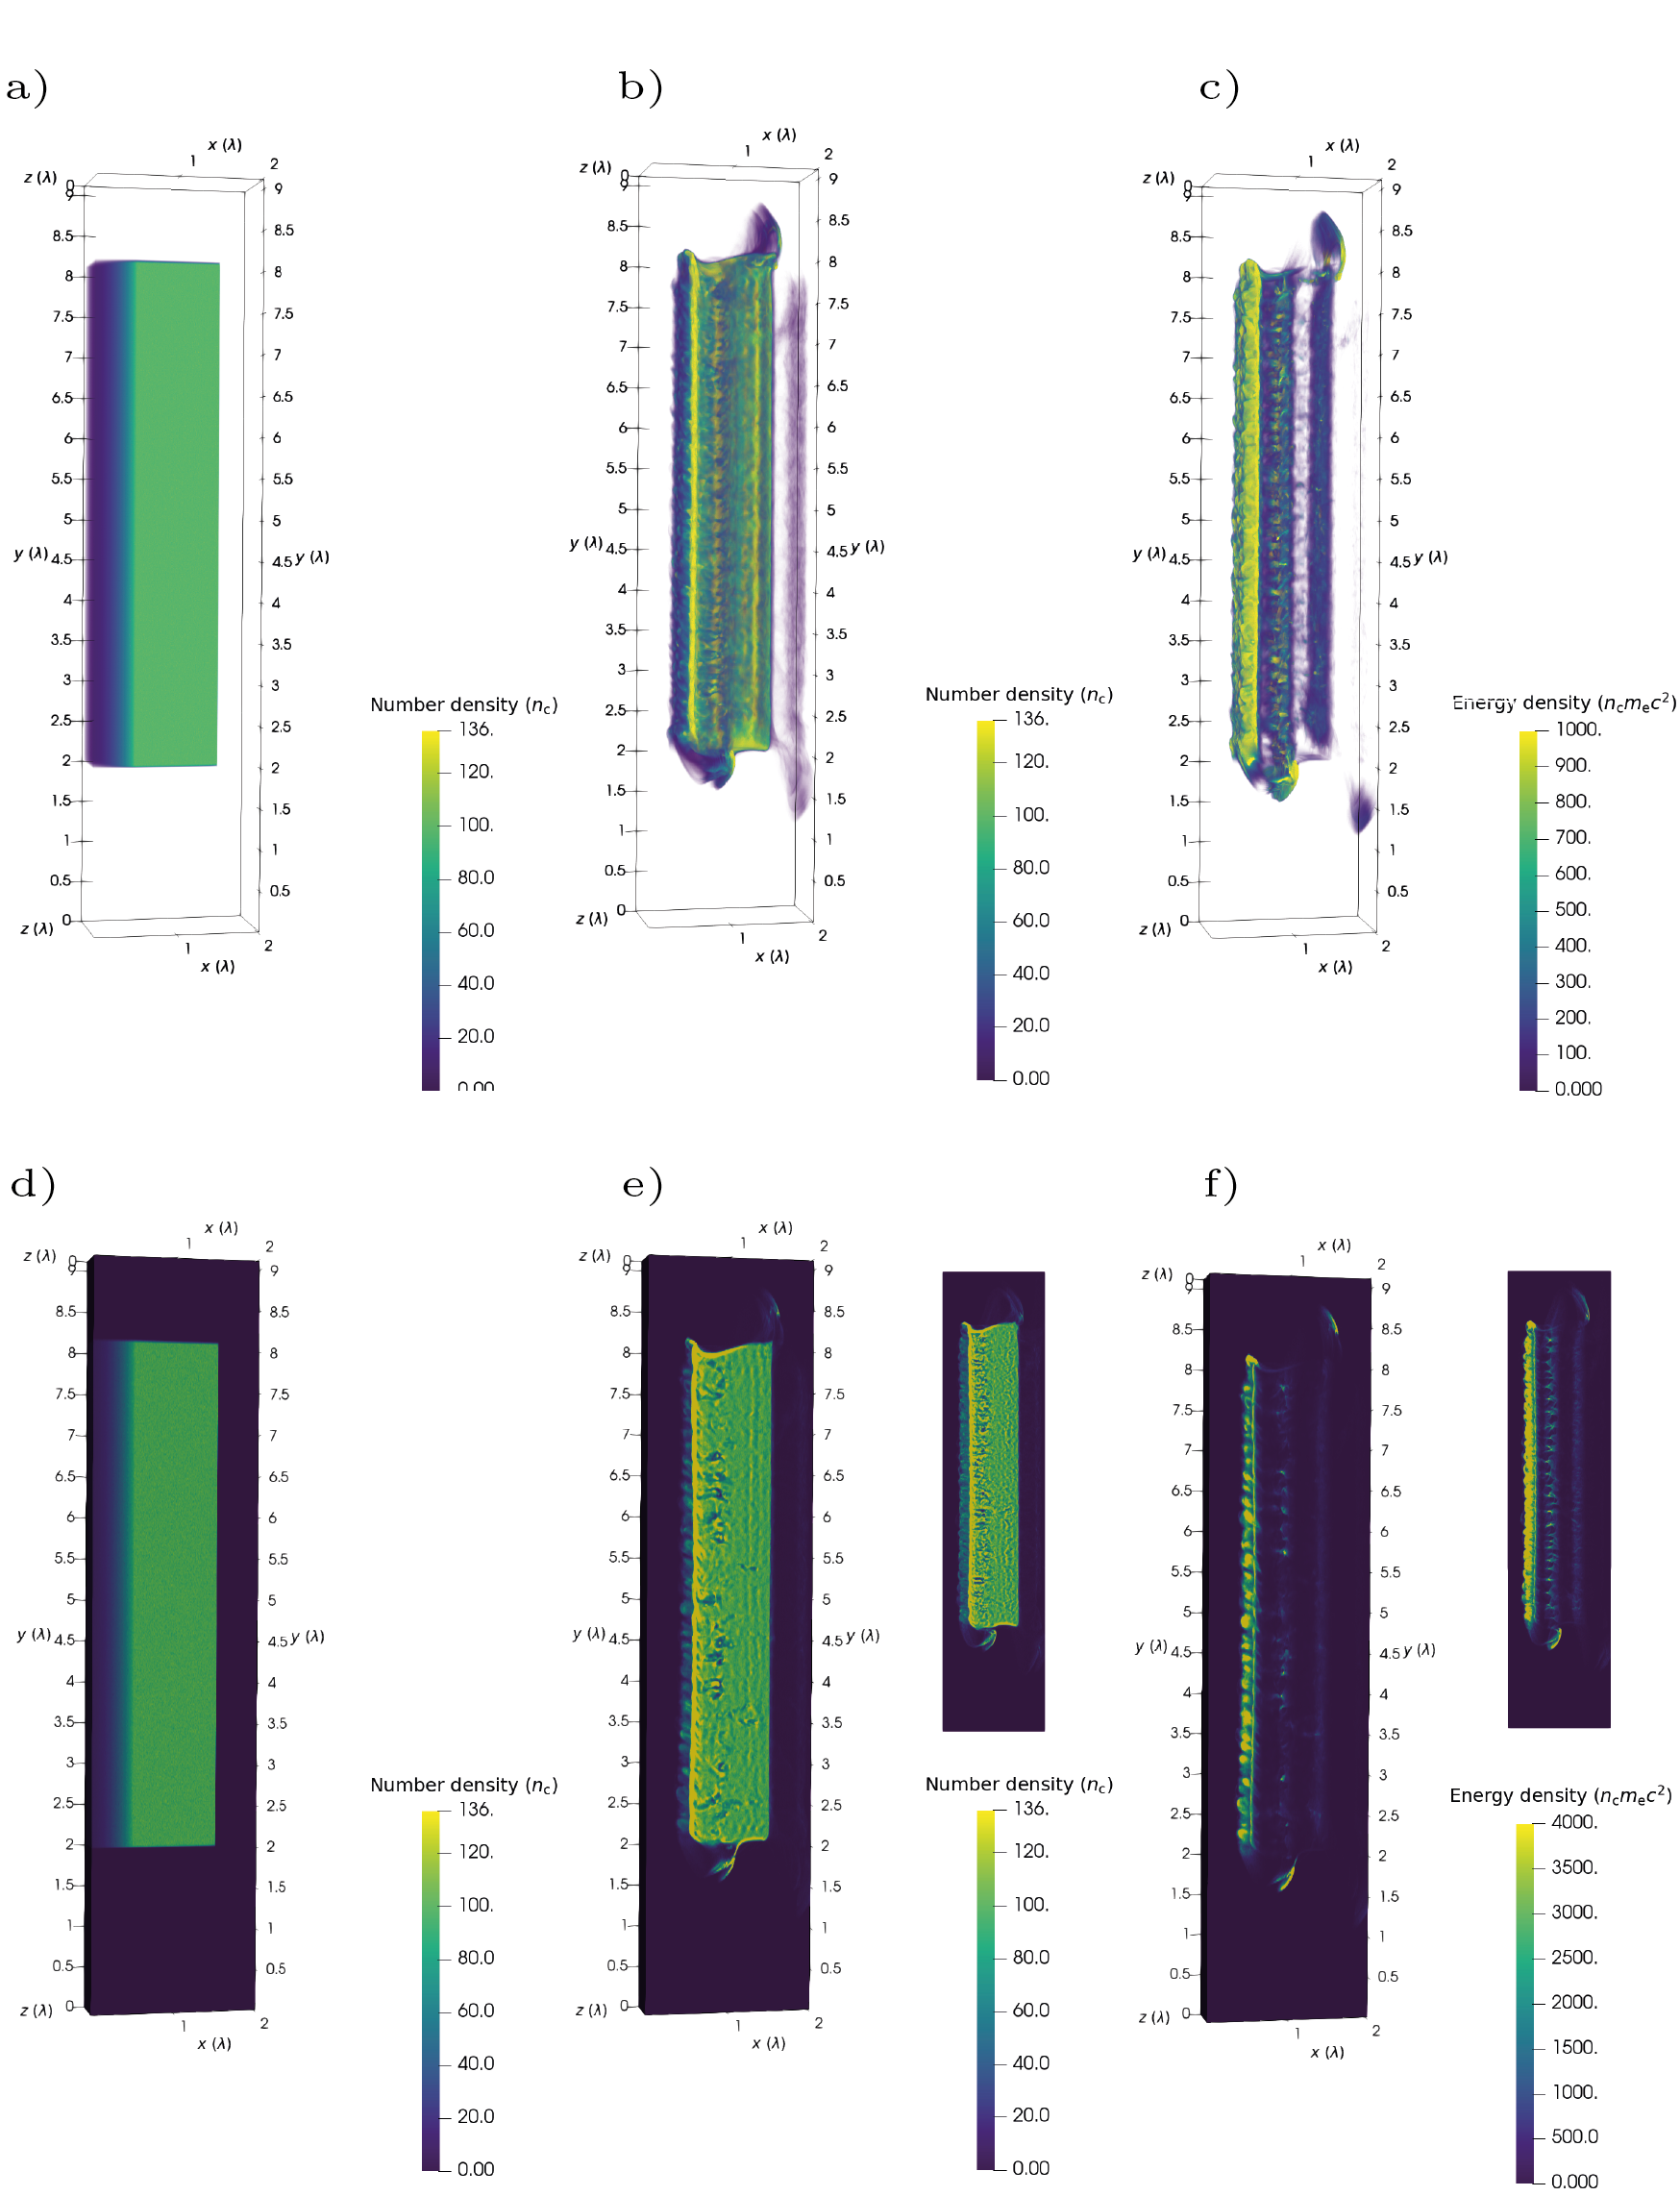
\includegraphics[width=1\linewidth]{figures/zvp/zvp_3D}
	\caption[Simulation results from a 3D \ac{PIC} simulation of the \ac{ZVP} mechanism. ]{Simulation results from a 3D \ac{PIC} simulation of the \ac{ZVP} mechanism. a) The initialised electron number density. b) The electron number density several cycles later, the plasma bulk is intact, however there is evidence of instabilities and electron bunches propagating through and around the plasma. c) The electron kinetic energy density at the same timestep. Note that the scale has been clipped to enable observation of both electron bunches propagating through and around the plasma bulk. Significantly higher energy density, corresponding to a higher charge density and attosecond duration for the electron bunches propagating around the bulk. d-f) Plots clipped through $z=\lambda_\mathrm{L}/2$ for a-c) respectively for better clarity on the internal structure of the plasma bulk. The accompanying plots for figures e) and f) are corresponding 2D PIC simulation results.}
	\label{fig:zvp3d}
\end{figure}
Simulation parameters are given in table \ref{tab:parameters}, such parameters are compatible with the 10 PW ELI-NP state-of-the-art short pulse laser facility \cite{tanakaCurrentStatusHighlights2020} and foam targets.
\begin{table}[]
	\begin{center}
	\begin{tabular}{lll}
		\hline \hline
		\multicolumn{3}{c}{Laser (3D, normal incidence)}   \\
		Parameters                                        & Real                                 & Sim                         \\ \hline
		Wavelength, $\lambda$ (nm)                        & 1060                                 & 2$\pi$                      \\
		Angular frequency, $\omega_\mathrm{L}$ (fs$^{-1}$)         & 1.8                                  & 1                           \\
		Beam waist, $w_\mathrm{L}$ (nm)                            & 6$\lambda$                           & 12$\pi$                     \\
		Focal point, ($x_f$, $y_f$, $z_f$) (nm)                  & (0.5$\lambda$, 5$\lambda$, $0.5\lambda$)             & ($\pi$, 10$\pi$, $\pi$)           \vspace{0.25cm}\\ 
		Spatial envelope, $E_i$, $i = y,z$                           & \multicolumn{2}{l}{$E_i \sim e^{-(i-i_f)^2/w_\mathrm{L}^2}$}                \\
		Temporal envelope, $E_t$                          & \multicolumn{2}{l}{$E_t \sim e^{-(t-4\lambda/c)^2/(4\lambda/3c)^2}$} \vspace{0.15cm}\\ \hline \hline
		\multicolumn{3}{c}{Simulation box}   \\ \hline
		Size, $x \times y\times z$ (nm)                           & $2\lambda \times 9\lambda \times \lambda$          & $4\pi \times 18\pi \times 2\pi$         \\
		Sim length (fs)                                   & 35.22                                & 20$\pi$                     \\
		Spatial resolution, $\Delta x$ (nm)               & $\lambda/128$ = 8.28                 & 0.0491                      \\
		Temporal resolution, $\Delta t$ (as)              & $\Delta x/11c$ = 2.51               & 0.00446                   \vspace{0.15cm}  \\ \hline \hline
		\multicolumn{3}{c}{Collisionless, pre-ionised randomly-initialised aluminium plasma}                                               \\ \hline
		Electron $x$ profile, $n(x)$                             & \multicolumn{2}{l}{$\begin{cases}
				n_\mathrm{e} \text{ for $2\lambda \le x \le 3\lambda$,}\\
				n_\mathrm{e}e^{(x-2\lambda)/0.2\lambda} \\
				\text{\hspace{0.5cm}for $x \le 2\lambda$.}\\
			\end{cases}$}                                               \\
		Electron $y$ profile, $n(y)$                              & \multicolumn{2}{l}{$\begin{cases}
				1 \text{ for $2\lambda \le y \le 8\lambda$,}\\
				0 \text{ otherwise.}\\
			\end{cases}$}                                               \\
		Electron $z$ profile, $n(z)$                              & \multicolumn{2}{l}{$\begin{cases}
		1 \text{ for $0.125\lambda \le y \le 0.875\lambda$,}\\
		0 \text{ otherwise.}\\
	\end{cases}$}                                               \\
		Ion profile, $n_\mathrm{i}(x,y,z)$                                & \multicolumn{2}{l}{$n_\mathrm{i} = n(x)n(y)n(z)/13$}                                                    \\
		Macro-electrons per cell                       & \multicolumn{2}{l}{729}                                                               \\
		Macro-ions per cell                               & 8                                   &  \\
		Ion temperature, $T_\mathrm{i}$ (keV)              &     0             &  0                         \\
		Electron temperature, $T_\mathrm{e}$ (keV)              &     10             &  0.02                          \\ \hline \hline
		\multicolumn{3}{c}{Stability criteria}                                               \\ \hline
		$\lambda_\mathrm{D}/\Delta x$                               &0.288                                   &  \\
		$1/\Delta t \omega_\mathrm{p}$                             &24.4                                   &  \\
		$\Delta x/c\Delta t$                             &   11                               &  \\
		Macro-particles in the Debye sphere                    &210                                  &  \vspace{0.15cm}\\ \hline \hline 

	\end{tabular}
	\end{center}
	\caption{\label{tab:parameters} \textbf{Simulation parameters in both real and normalised Smilei simulation units for the 3D3V simulations.} }
\end{table}
Figure \ref{fig:zvp3d}c) clearly demonstrates the existence of high energy density electron bunches propagating through the plasma bulk in the direction of the laser pulse. Note that this ZVP criterion is a direct consequence of conservation of transverse momentum inside the plasma bulk where the laser fields cannot propagate. Figure \ref{fig:zvp3d}b) shows these bunches escape to the rear of the bulk but lose energy as they do so. Looking now at figure \ref{fig:zvp3d}e) and the internal structure of the plasma bulk. These bunches drive two-stream and filamentation instabilities \cite{bretMultidimensionalElectronBeamplasma2010}. The bulk propagating bunches are accompanied by higher density electron bunches to either side of the plasma block with the side switching every half laser pulse cycle. 

The thickness of the target does not impact the interaction and is chosen for computational efficiency, indeed it is standard to consider such targets of thickness $\ge \lambda_\mathrm{L}$ as bulk targets \cite{dollarEnhancedLaserAbsorption2017}, however, for sufficiently long pulse durations, the effect of hole boring necessitates thicker targets to make this approximation as will be required in the following chapter.

For the 3D simulations only, particles were initialised randomly instead of regularly to avoid numerical errors. Regularly initialised plasma blocks in 3D simulations blow apart very quickly due to spurious large amplitude fields generated on the large plasma surface due to macroscopic electron-ion charge separation at initialisation. 2D simulations with randomly initialised particles tend to produce nano-structures reminiscet of cosmic filaments. This would appear erroneous as it is not present in equivalent 3D simulations and is likely due to the lack of degrees of freedom available in the system. This error can be reduced by increasing the plasma temperature.

The plasma specifications were chosen to minimise computational load while ensuring numerical convergence, requiring over 100 billion macroparticles. The electron temperature is raised significantly higher than that which would be expected in such a laser-plasma system so as to resolve the Debye length. Anticipated plasma temperatures are calculated using 1D HYADES simulations in the following chapter. While this temperature is unphysical and will lead to some small plasma expansion over the course of the simulation, the temperature remains negligible compared to that imparted to the electron bunches by the laser pulse. The striking similarity between the 2 and 3D simulation results is a natural consequence of the 2D nature of the interaction geometry. It is, however, still reassuring to show that previous work withstands the stringent test of real universe geometry and the ZVP mechanism is not lost in the chaos.

\subsubsection{Convergence of 3D simulations}
The 3D simulation parameters were chosen to be consistent with previous work on the \ac{ZVP} mechanism, however, such simulations are cumbersome, limiting the number of simulations it is feasible to run. In order to query the defining characteristics outlined by Baeva, a lower resolution simulation was performed with similar parameters to the initial simulation. Comparisons between the simulation outputs are made in figure \ref{fig:zvp3dcomparelowres} in appendix \ref{sec:app-pic_convergence3D}. Good convergence is qualitatively demonstrated by the presence of characteristic features of the ZVP mechanism. While the instabilities are similar in structure, the change in seeding changes their exact positions. As instabilities are not the focus of this thesis this variation is of no cause for concern, however, while the characteristics remain similar, some caution must be taken with any quantitative results.

\subsubsection{Confirmation of ZVP in 3D}
Figure \ref{fig:zvppropagatingzero} tracks the transverse momentum distribution along the polarisation axis of the laser pulse of an electron bunch during its ablative journey, clearly demonstrating the existence of a singular zero of the vector potential propagating through the electron bunch and away from the plasma bulk.

\begin{figure}
	\centering
	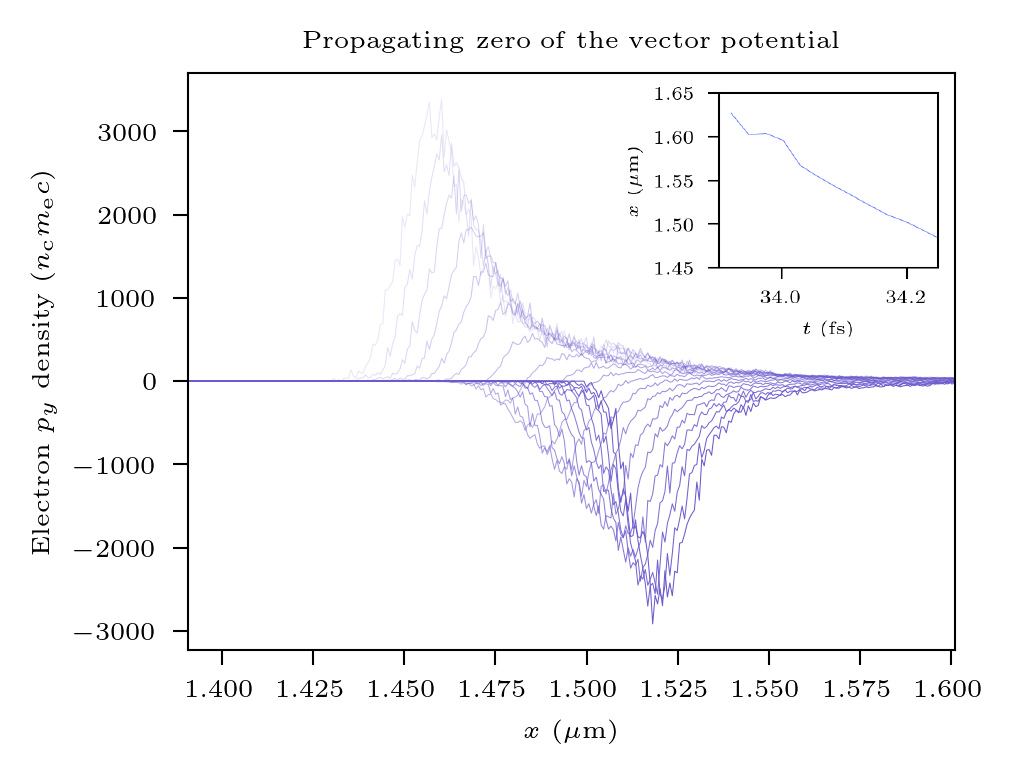
\includegraphics[width=0.7\linewidth]{figures/zvp/zvp_propagating_zero}
	\caption[Propagation of zeroes through the ablating ZVP electron bunch.]{Propagation of zeroes through the ablating ZVP electron bunch via the proxy of tranverse momentum conservation. The zero of the vector potential exists where the transverse momentum is macroscopically zero. Each line represents a timestep with time increasing with decreasing colour. With increasing time the bunch and the zero move in the -$\hat{\mathbf{x}}$-direction with the zero overtaking the electron bunch. The inset tracks the position of the zero of the vector potential with time.}
	\label{fig:zvppropagatingzero}
\end{figure}
The zero propagates at a speed of $\approx 1.4c$. In this simulation, the zero propagates through the bunch before it finishes crossing the pseudocapacitor and thus before it has acquired its maximum velocity. As previously discussed this reduces the coherency of the emitted radiation, this provides a new perspective from which to consider optimisation of HHG.

Further simulation results a presented in figure \ref{fig:zvp3ddynamics}.

\begin{figure}
	\centering
	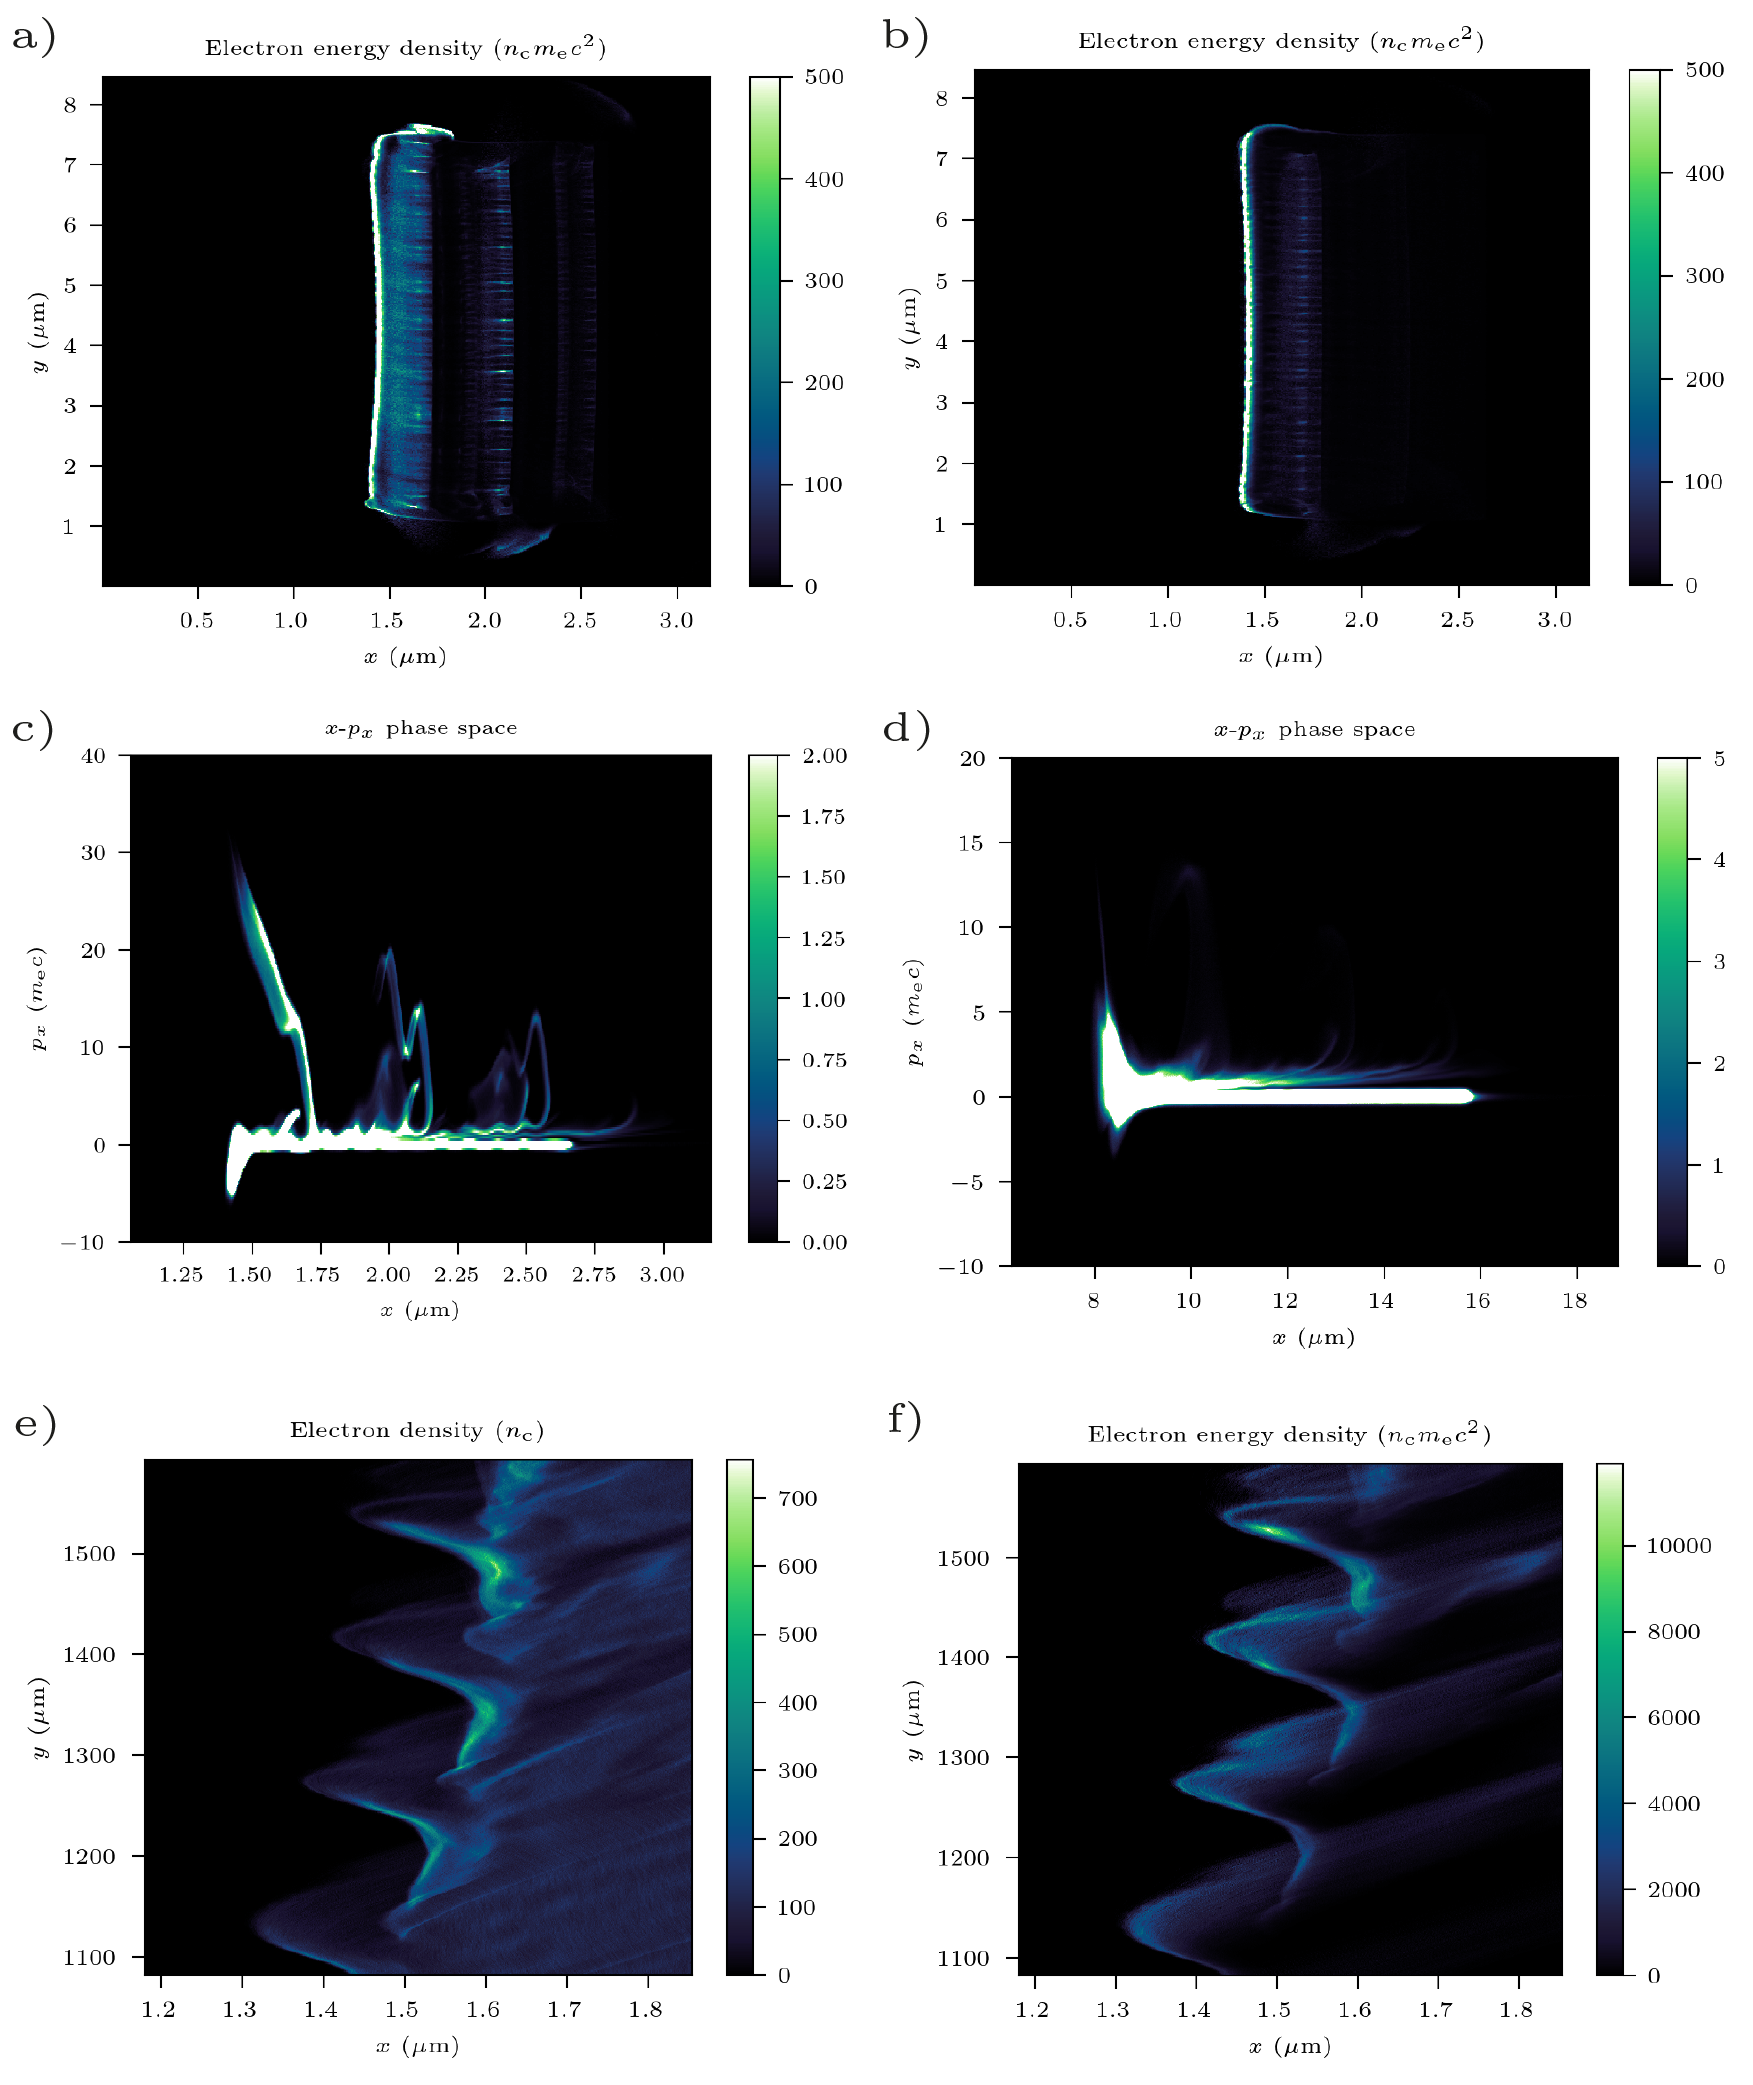
\includegraphics[width=1\linewidth]{figures/zvp/zvp_3D_dynamics}
	\caption[Electron dynamics in 3D PIC simulation for both linear and cirularly polarised relativistic laser pulses.]{Electron dynamics in a 3D PIC simulation. a) and b) Electron energy density for linearly and circularly polarised laser pulses respectively. c) and d) Electron longitudinal momentum for linearly and circularly polarised laser pulses respectively.  e) Electron density at the plasma surface streaked in time. f) Electron energy density at the plasma surface streaked in time.}
	\label{fig:zvp3ddynamics}
\end{figure}
In figures \ref{fig:zvp3ddynamics}a)-d), comparisons are made in the electron energy distributions for simulations with zeros present in the vector potential (linearly polarised) and without (circularly polarised). Clearly zeroes are required for the formation of high energy, short duration attosecond bunches. From figure \ref{fig:zvp3ddynamics}a) it is clear that electron bunches are injected and propagate through the plasma bulk in the laser propagation direction. Figure \ref{fig:zvp3ddynamics}c) demonstrates the quasi-monoenergeticity of the high energy electron bunches as initially identified in 1D by Baeva. Although the shape in the phase space is more complex in 3D, the attosecond duration at a given energy is retained. Figures \ref{fig:zvp3ddynamics}e) and f) describe the surface dynamics. One can observe the high density bunches on the front surface with the peak in energy density occuring after acceleration across the pseudocapacitor. Figure \ref{fig:zvp3ddynamics}f) also explains the shape of the spectrum of figure \ref{fig:zvp3ddynamics}c), low energy electrons are turned back first and as all bunch electrons are ultrarelativistic, the higher energy electrons trail behind.

Finally, figure \ref{fig:zvphhgbeamfourier} compares the spectra of the reflected light in the presence and absence of zeros of the vector potential.
\begin{figure}
	\centering
	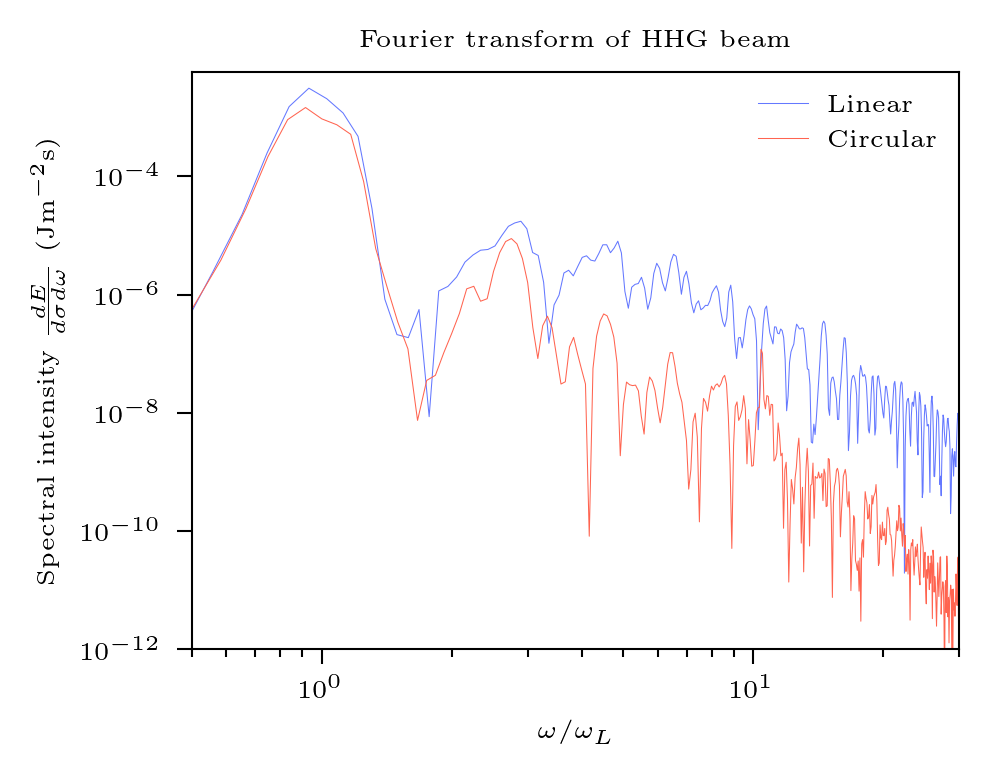
\includegraphics[width=0.7\linewidth]{figures/zvp/zvp_hhg_beam_fourier}
	\caption[The Fourier transform of the reflected laser pulse in 3D PIC simulations.]{The Fourier transform of the reflected laser pulse in 3D PIC simulations both with and without zeroes in the vector potential.}
	\label{fig:zvphhgbeamfourier}
\end{figure}
Unfortunately the simulation resolution is too low to resolve the individual harmonics however, the spectrum from the circularly polarised light is typically over two orders of magnitude below that for linearly polarised light. Thus, all defining characteristics of the ZVP mechanism have been identified in 3D simulations with the notable exception of the energy scalings. Next generation supercomputers will be required to perform such parameter scans.

% TODO: \textbf{**To do: these dynamics plots need fixing. Should add the times, also e and f have distance instead of time on y axis, also need to convert from timstep to time. D) needs teh scale changing. also the x axis needs converting to distance. Also to do I need to change the colour of that FFT graph**}

\section{The ZVP electron bunch}\label{sec:zvp-bunches}
Following the success in reproducing the key features of the \ac{ZVP} mechanism and demonstrated consistency between 2 and 3D equivalent simulations, the remainder of this chapter will predominantly utilise 2D simulations to interrogate the interaction further. Previous work on the ZVP mechanism has highlighted the high energy and short duration of electron bunches, now full characterisation of such bunches is performed. A ZVP electron bunch is an electron bunch produced via the ZVP mechanism. Once produced and accelerated across the pseudocapacitor field, it is launched back in the laser propagation direction. While the bunch has no spatial separation over energies when propagating with the zero of the vector potential, the turning point of the electrons is longitudinal momentum dependent due to the Coulomb attraction of the ions after overshooting the pseudocapacitor field. Baeva \textit{et al} showed that the electron bunch has a quasi-monoenergetic spectrum: there is a one-to-one relationship between energy and position with the higher energies trailing the lower energies. The full bunch is confined to 130 as while a single energy confined to 5 as. If, however, the plasma bulk is transversely mass-limited relative to the laser spot size,when rotated back towards the plasma block, some of the electron bunch will overshoot and escape the potential well without significant stretching of the bunch in time as can be seen in figure \ref{fig:zvp3d}. Such electron bunches retain their high charge density and ultra-short duration. ZVP electron bunches can therefore be placed into two categories: ultra-high charge, ultra-short duraction electron bunches from mass-limited targets, hereafter labelled mass-limited electron bunches, of interest due to their unique properties, and bulk propagating bunches, hereafter labelled bulk bunches, which have lower charge densities, are imprinted with instabilities and are instead of interest due to their connection to energy absorption and reflection in this post-ponderomotive regime. To investigate these two bunch types further, 2D PIC simulations were performed, see appendix for parameters.
 
 \subsubsection{Attosecond nano-Coulomb mass-limited electron bunches}
 Figure \ref{fig:zvptypicalbunch} describes a typical mass-limited ZVP electron bunch qualitatively.
\begin{figure}
	\centering
	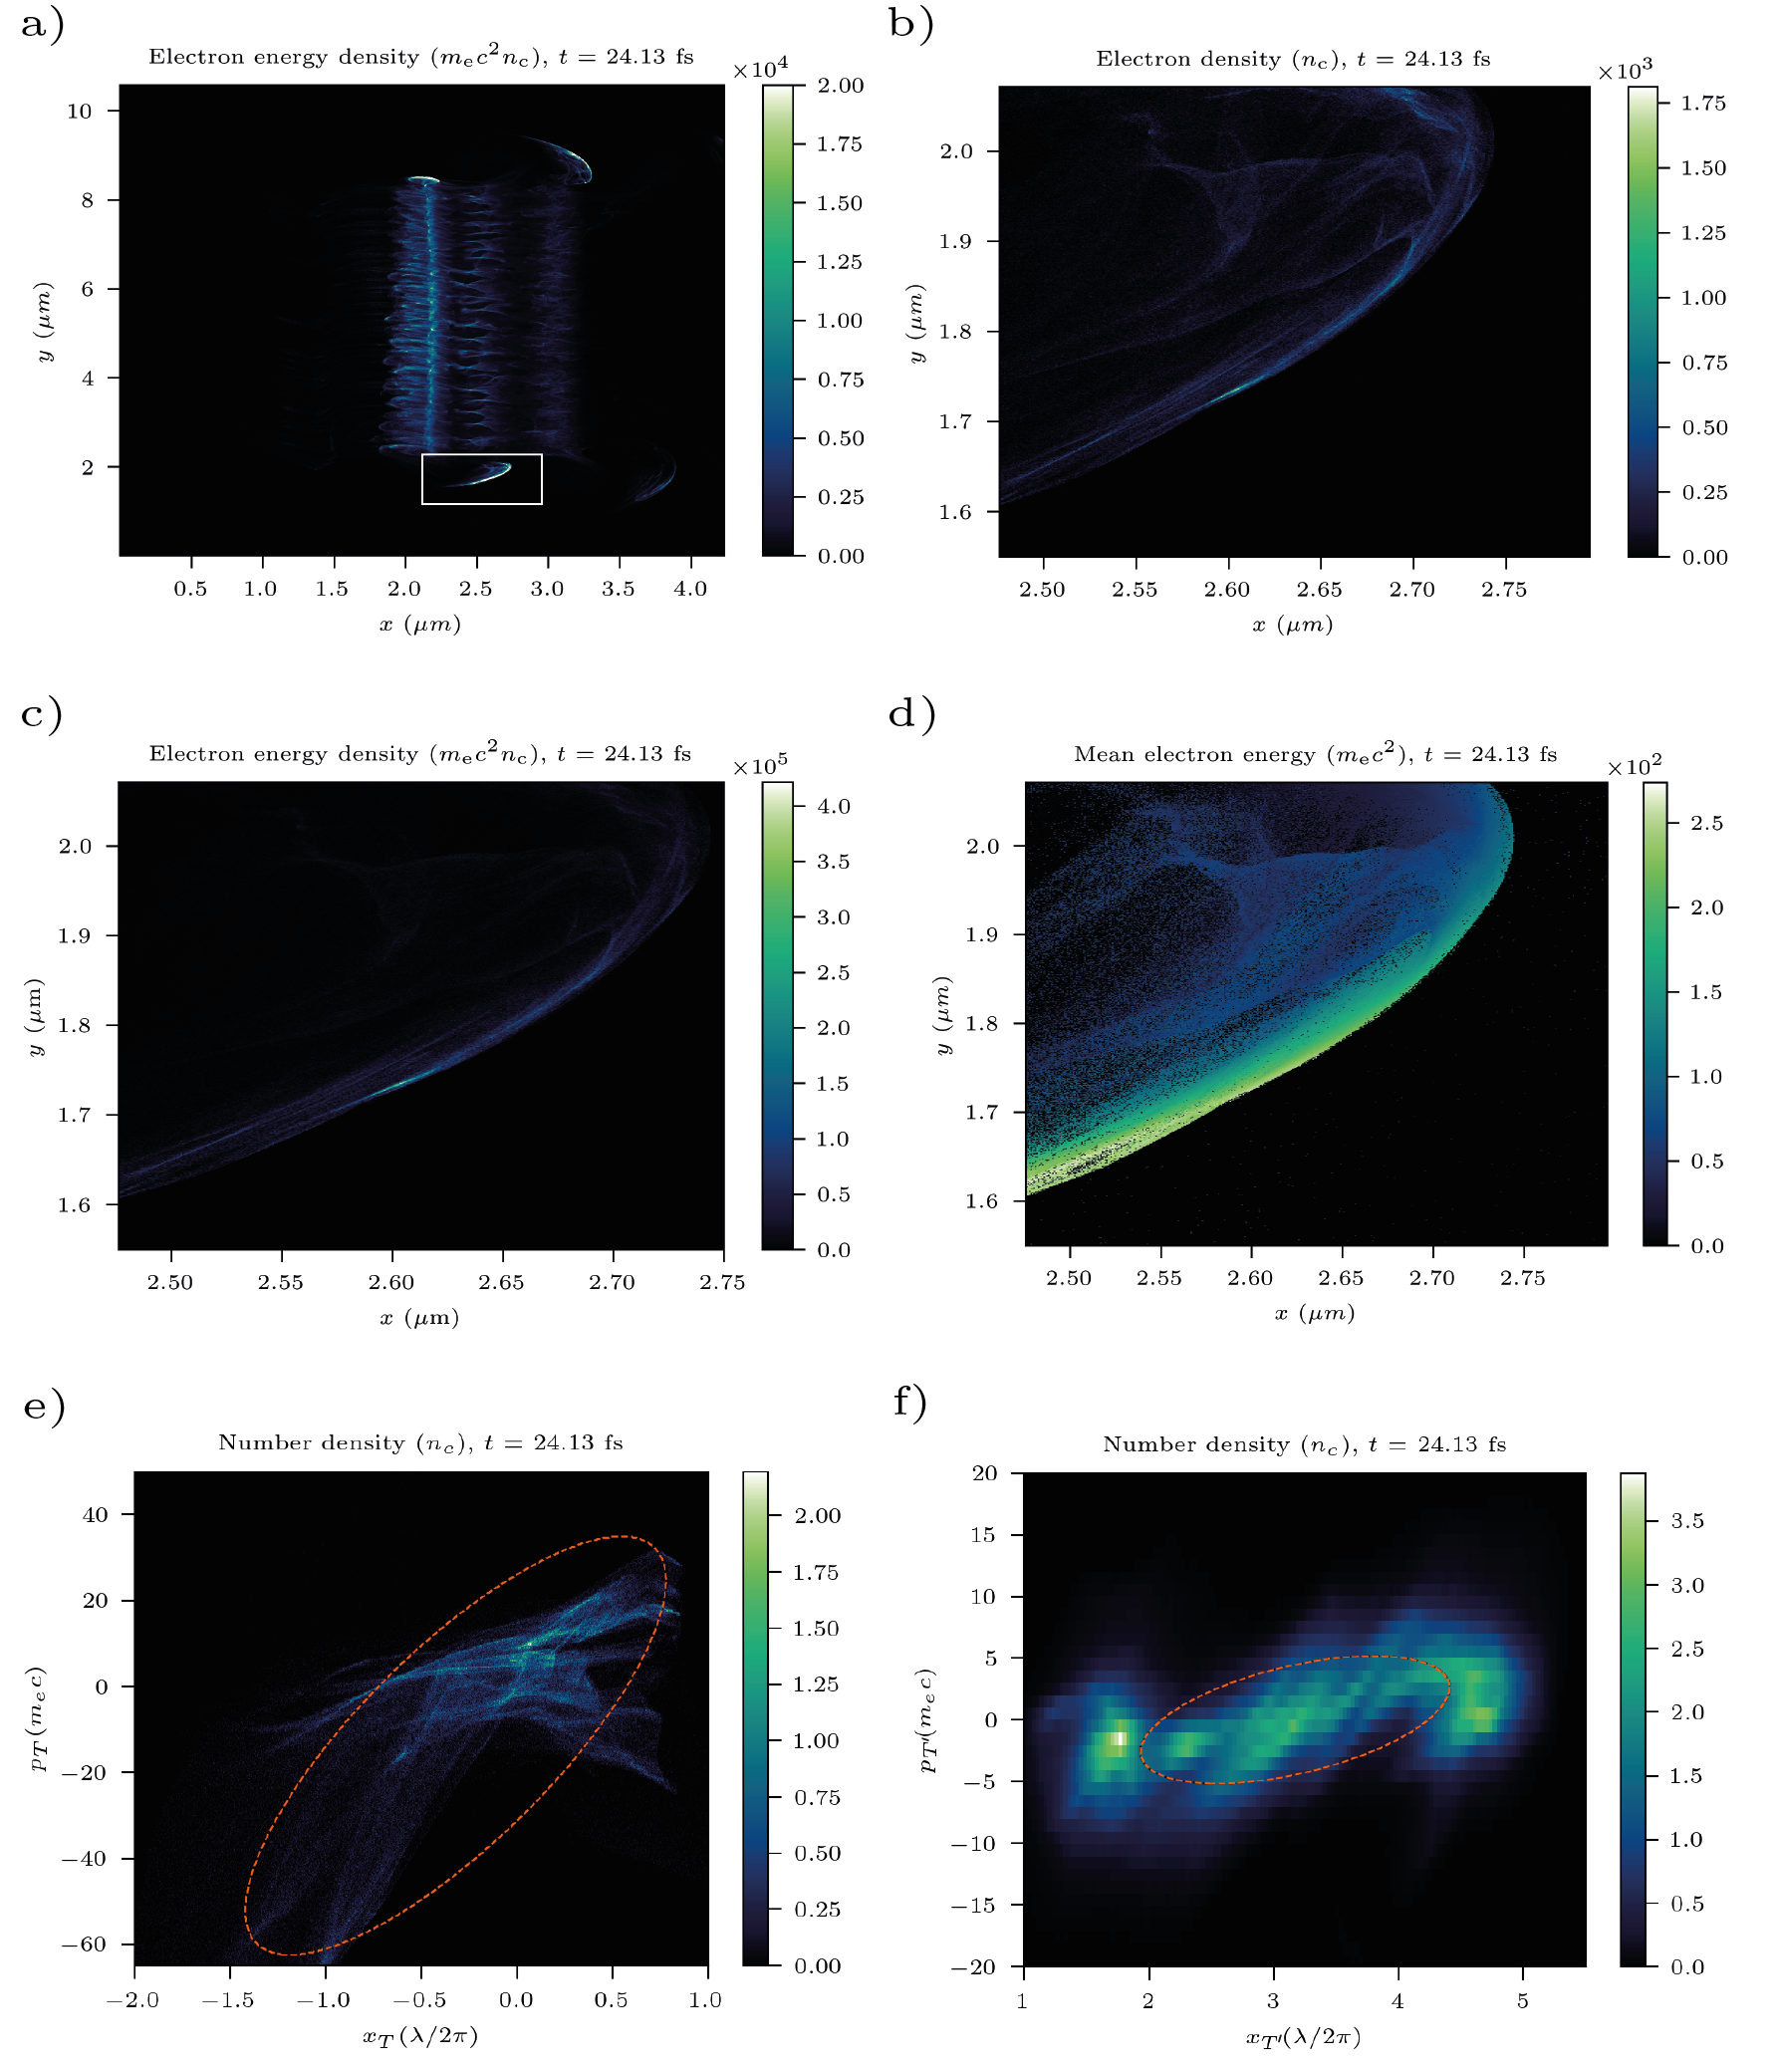
\includegraphics[width=1\linewidth]{figures/zvp/zvp_typical_bunch}
	\caption[2D PIC simulation results qualitatively describing typical mass-limited ZVP electron bunch structure.]{2D PIC simulation results qualitatively describing typical mass-limited ZVP electron bunch structure. a) Electron energy density for the full simulation window, corresponds to figure \ref{fig:zvp3d}f).  The box highlights the bunch presented in the following plots. b) Electron number density of the electron bunch. c) Electron energy density of the electron bunch, the colourbar scale has been increased compared to figure a) to demonstrate the internal structure. d) The mean electron energy across the electron bunch, suggesting a position dependent energy or quasi-monoenergetic nature to the electron bunch \cite{baevaZeroVectorPotential2011}. Cells with no macroparticles are black. e) The transverse phase space in the 2D simulation plane. The ellipse describes the calculated emittance. The skew of the ellipse is a consequence of a low density tail on the phase space beyond the bottom left corner. f) This plot was extracted from the equivalent 3D simulation and describes the transverse emittance in the $z$-direction. Again the ellipse marks the emittance. The relatively well-defined border to the phase space and the mild tilt (indicating only mild divergence) are direct consequences of the 2D nature of the interaction.}
	\label{fig:zvptypicalbunch}
\end{figure}
The electron bunch under interrogation is ultra-relativistic with a mean energy of \qty{51\pm 11}{MeV} and a duration of 35 as. It propagates at an angle of -393 rad relative to the laser propagation direction, \textit{i.e.} the $x$-axis, and has a transverse geometric emittance in the simulation plane (the $x$-$y$ plane) of \qty{35 \pm 7}{nm.rad}. The calculation of the transverse geometric emittance, a measure of the quality of the electron beam, is given in appendix \ref{app:1-basics-transverse_emittance}. Note that while the bunch does not propagate in the laser propagation direction, this does not mean it must be rejected under consideration of the ZVP bunch conditions. Indeed, the bunch must propagate at some angle to the laser due to conservation of canonical momentum while it remains in thrall of the laser pulse. For an equivalent bunch in a corresponding 3D simulation, the transverse geometric emittance in the $z$ plane is \qty{15\pm 11}{nm.rad}. This electron bunch has a total charge of 0.35 nC for a slab of plasma of thickness $0.75\lambda$ in the $z$-direction. Noting again the two-dimensional nature of the interaction geometry, and that electrons less than twice the relativistic Larmor radius, 
\begin{equation}
	r_\mathrm{L} = \frac{\gamma m_\mathrm{e}v}{e|\mathbf{B}|},
\end{equation}
where $\gamma$ and $v$ correspond to the electron velocity, when rotated back towards the plasma will escape to the side, the total number of electrons in the mass-limited bunch is
\begin{equation}
	N = 2 n_\mathrm{e} r_\mathrm{l} L_z \Delta x,
\end{equation}
where $L_z$ is the width of the plasma in the $z$-direction. Using equation \ref{eq:zvp_dx} for $\Delta x$ and \ref{eq:zvp_gamma} for $\gamma$ and approximating $v \approx c$ for the ultra-relativistic electron bunch, 
\begin{equation}\label{eq:zvp_N}
	N = 2 \gamma n_\mathrm{c} \frac{L_z}{k^2}.
\end{equation}
For these simulation parameters, this corresponds to a total bunch charge, $Q = eN$, of 0.37 nC, a remarkably successful prediction of the ZVP model. Equation \ref{eq:zvp_N} tells us there is no limit to the 

Equation \ref{eq:zvp_N} can be rewritten in terms of fundamental constants as
\begin{equation}\label{eq:zvp_N2}
	N = 2 (1+0.5\frac{a^2_0}{\bar{n}_\mathrm{e}}) L_z \frac{m_\mathrm{e}\epsilon_0c^2}{e^2}.
\end{equation}
Counter-intuitively, it would appear the total charge scales inversely with the plasma density. Instead, charge can be increased either by increasing the laser pulse intensity or $L_z$. Indeed, provided the laser pulse intensity remains relativistic, the focal spot can be increased indefinitely and there is no limit to the mass-limited electron bunch total charge. For a realistic laser pulse with beam width $10 \lambda$ incident on a larger laser block, equation \ref{eq:zvp_N2} predicts a charge of 9.3 nC.

Figure \ref{fig:zvptypicalbunchlines}a compares the electron bunch energy to an equivalent bunch produced by a circularly polarised laser pulse\footnote{A circularly polarised laser pulse will expel electrons from a mass-limited target in a corkscrew shape, the bunch is therefore only loosely equivalent.}. The mean electron bunch energy is over three times lower as there is no ZVP acceleration phase and there is no quasi-monochromatic structure \cite{baevaZeroVectorPotential2011}. Figure \ref{fig:zvptypicalbunchlines}b demonstrates the attosecond duration of the electron bunch.
\begin{figure}
	\centering
	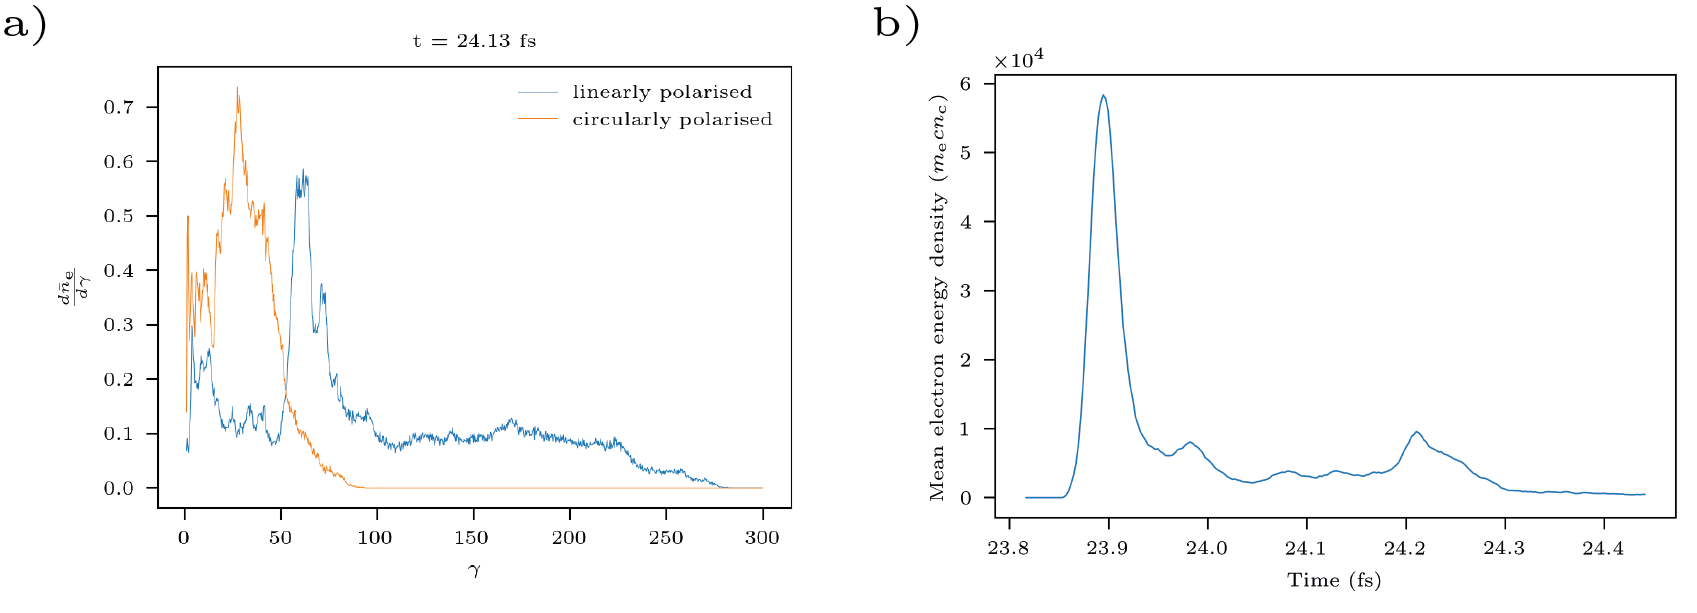
\includegraphics[width=1\linewidth]{figures/zvp/zvp_typical_bunch_lines}
	\caption[Energy spectra for mass-limited electron bunches formed via linearly and circularly polarised laser pulses.]{a) Energy spectra for mass-limited electron bunches formed via linearly and circularly polarised laser pulses. b) Mean energy density streaked in time through the centre of a mass-limited ZVP electron bunch demonstrating the attosecond duration.}
	\label{fig:zvptypicalbunchlines}
\end{figure}

\subsubsection{Applications: from electron bunches to attosecond light}
There are a plethora of applications for high charge, attosecond electron bunches, primarily enabling the resolution of attosecond scale phenomena \cite{krauszAttosecondPhysics2009}. Already femtosecond pump, attosecond probe experiments are underway \cite{calegariUltrafastElectronDynamics,takahashiNonlinearAttosecondMetrology2015} but the higher intensities and charge densities accessible in the laser-solid regime compared to laser-gas interactions \cite{edwardsXRayEmissionEffectiveness2020, linIsolatedAttosecondElectron2020} would dramatically advance the field by enabling atto-pump atto-probe experiments \cite{zhangGiantIsolatedAttosecond2020}. Potential applications include: electron microscopy and atomic diffraction to temporally resolve photoelectric processes such as Bragg diffraction \cite{morimotoDiffractionMicroscopyAttosecond2018}, ultra-fast electron radiography to probe the evolution of the formation of magnetic fields in dynamical systems \cite{schumakerUltrafastElectronRadiography2013} or for XFEL seeding \cite{cardenasSubcycleDynamicsRelativistic2019}: the record XFEL X-ray pulse duration stands at 280 attoseconds \cite{durisTunableIsolatedAttosecond2020}, substantially longer than the durations accessible using this technique. Electron bunches are also a promising alternative for radiotherapy due to their superior penetration depth in biotissues compared to X-rays \cite{glinecRadiotherapyLaserPlasma2006}.

Analogously to the \ac{HHG} process, rapid acceleration of an electron bunch generates a burst of radiation whose properties (brightness, coherency, duration, spectrum) are determined by the corresponding properties of the electron bunch (charge, emittance, duration and energy). Thus globally electron bunches are used as a diagnostic tool in synchrotrons and XFELs. Other acceleration mechanisms for X-ray generation include: bremmstrahlung radiation from firing the electron bunch at a secondary high-$Z$ target \cite{cordeFemtosecondRaysLaserplasma2013}, interaction with a counter-propagating laser pulse \cite{khrennikovTunableAllOpticalQuasimonochromatic2015,kulaginNonlinearReflectionHighamplitude2016} or injection into a laser or plasma wakefield accelerator\textbf{CITE}, including accessing the solid density plasma wakefield regime \cite{linIsolatedAttosecondElectron2020}. The mass-limited electron bunches produced via the ZVP mechanism have transverse emittances comparable in all planes to those conditioned in state-of-the-art nano-Coulomb electron bunch accelerators \cite{martinDiamondLightSource2020,pingProgressHEPSProject2020}. Such facilities typically produce electron bunches with geometric emittances of $\sim \unit{mm.rad}$ prior to damping ring injection \cite{christouPreInjectorLinacDiamond2004} and $\sim \unit{nm.rad}$ post-injection \cite{martinDiamondLightSource2020}. Thus, the mass-limited ZVP electron bunches are ideal candidates for the production of bright X-rays of unprecedentedly short duration and are suitable for the study of the new regime of attosecond science with applications to physical, chemical and biological systems.

\subsubsection{Parameter scan of electron bunch mean energy}
Since ZVP energy scaling is a fundamental identifier of ZVP bunches, it is important to confirm that mass-limited electron bunches follow the same scaling relations as has previously been confirmed for bulk ZVP electrons in both 1D \cite{baevaZeroVectorPotential2011} and 2D \cite{savinAttosecondscaleAbsorptionExtreme2017} PIC simulations. The mean mass-limited electron bunch kinetic energies were extracted from 120 2D PIC simulations and are plotted in figure \ref{fig:zvpmeangammas}. 
\begin{figure}
	\centering
	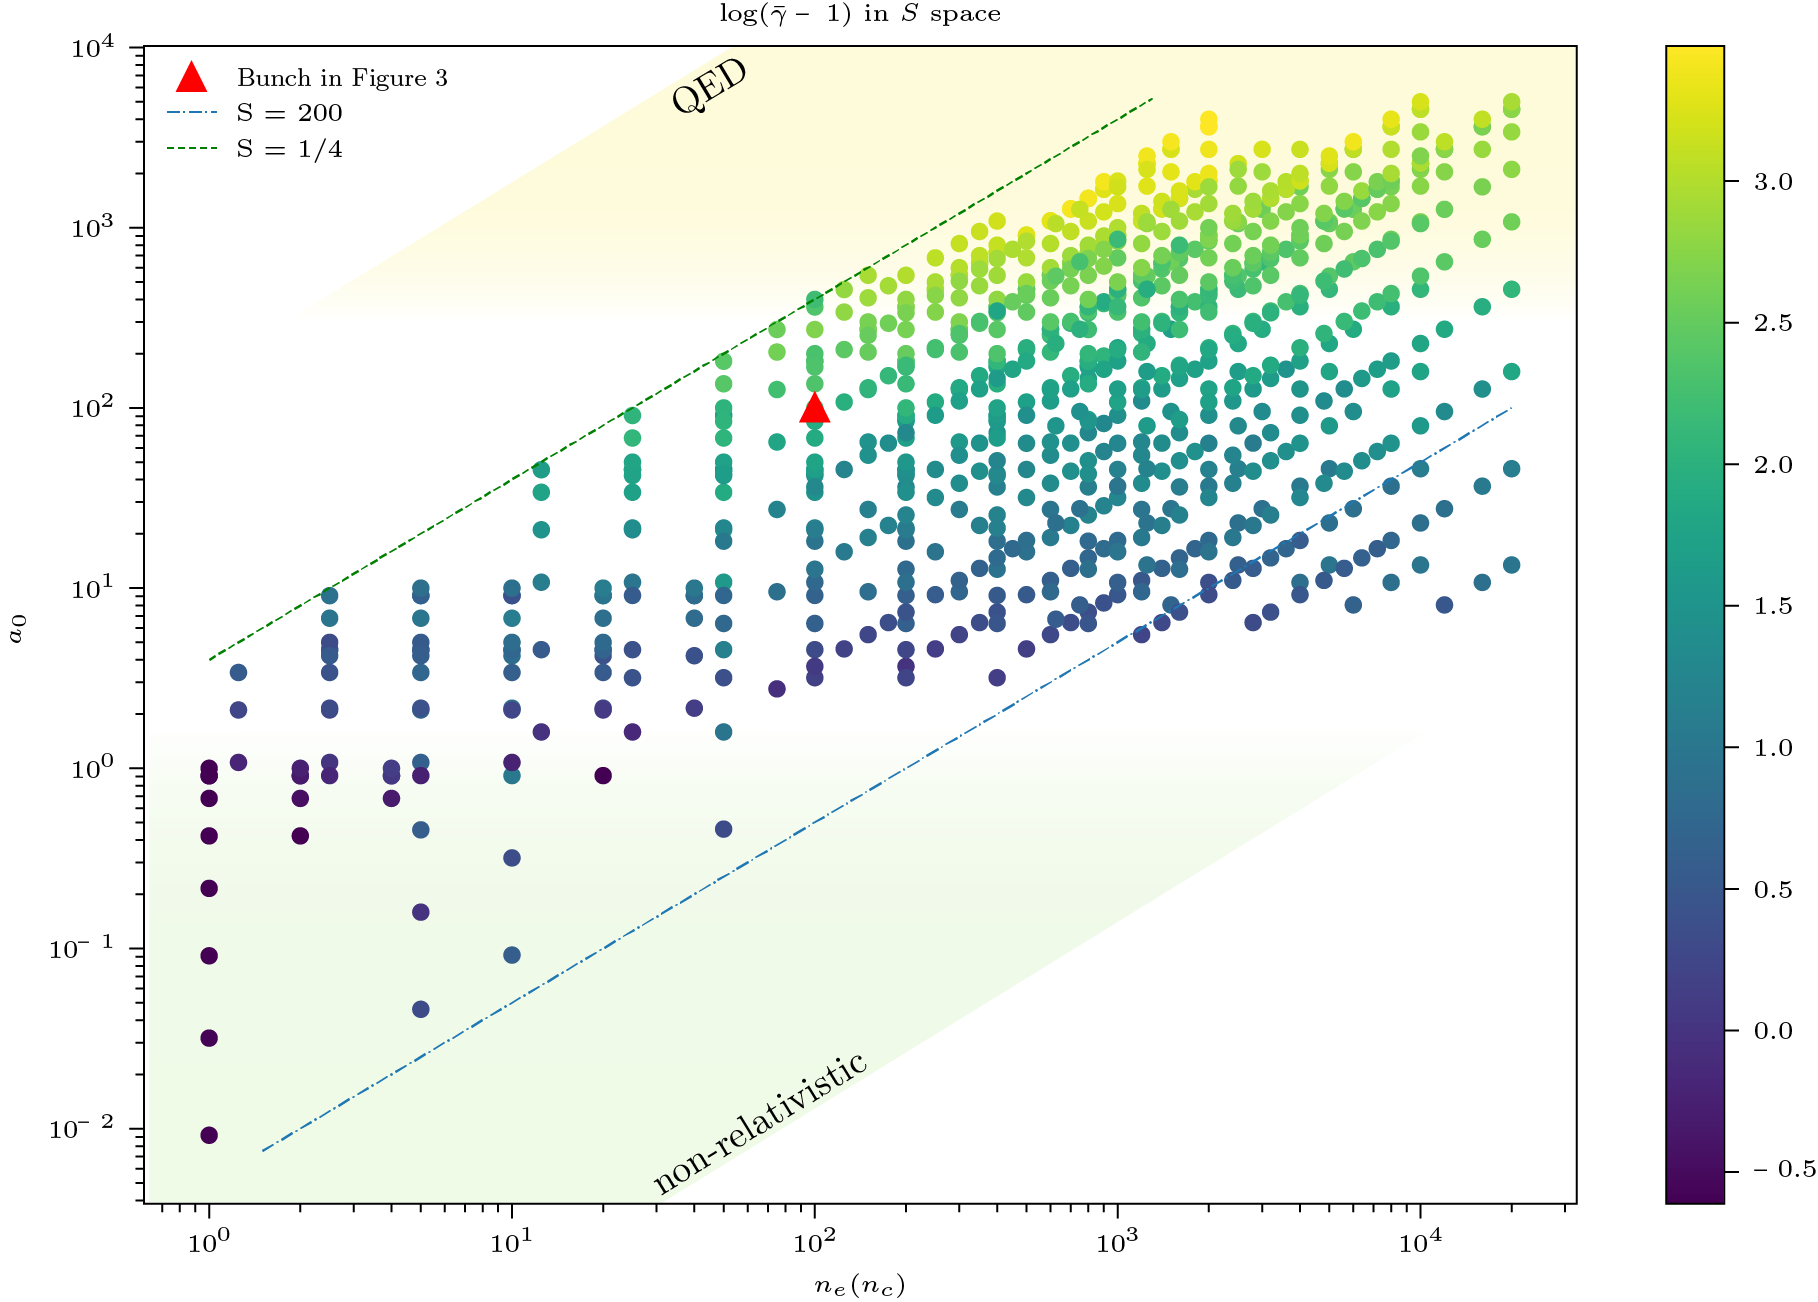
\includegraphics[width=1\linewidth]{figures/zvp/zvp_mean_gammas}
	\caption[Mean mass-limited ZVP electron bunch normalised kinetic energies extracted from 2D PIC simulations.]{Mean mass-limited ZVP electron bunch normalised kinetic energies extracted from 2D PIC simulations. The bunch detailed in figure \ref{fig:zvptypicalbunch} is highlighted.}
	\label{fig:zvpmeangammas}
\end{figure}
Particle merging was turned on for macro-photons and macro-electrons for $a_0 \ge 1800$ to prevent overloading of the available supercomputer memory due to the vast number of particles produced in this SF-QED regime. The dependence on both $a_0$ and $n_\mathrm{e}$ demonstrates these electron bunches are accelerated by a non-pondermotive mechanism. The parameter scan took plasma block densities ranging from the critical plasma density to well-beyond solid density for the aluminium target and with laser pulse peak intensities ranging from non-relativistic ($a_0 < 1$) through to the \ac{QED} plasma regime ($a_0 > 300$) up to a peak $a_0 = 5000$ to investigate the change in scaling observed by Savin \textit{et al} \cite{savinEnergyAbsorptionLaserQED2019} at the onset of QED effects. This study is also the first to extract specific bunch energies as opposed to total simulation box energy gain, representing a far more focused test of ZVP theory.

Care must be taken however as the energy of such electron bunches cannot be directly compared to the ZVP energy relations as as aforementioned, after escaping the potential, the electron bunch experiences further direct laser acceleration before reaching the detection point. Indeed, Thévenet \textit{et al} \cite{thevenetVacuumLaserAcceleration2016} suggested that attosecond electron bunches produced in reflection exhibit precisely the phase and energy properties required to `surf' the reflected laser pulse and experience vast acceleration gradients over the Rayleigh length of the laser pulse. This process is known as Vacuum Laser Acceleration. It seems highly likely that this process occurs for electron bunches produced in transmission. This seemingly unfortunately situation in reality provide a fully optical scheme to create GeV nano-Coulomb electron bunches from the most basic of setups: a laser and a solid density target.

Returning to the determination of the electron bunch energy at the measurement point, consider now the journey of the electron bunch after expulsion from the plasma bulk. It is rotated back towards the plasma bulk by the magnetic field of the subsequent peak of the laser pulse, then travelling at approximately $c$ it surfs the peak, experiencing an approximately constant accelerating electric field from the laser pulse at some fraction $f$ of the laser field peak. The work done by this field is then
\begin{equation}
	\Delta T = \int e \mathbf{E} \cdot \mathrm{d}\mathbf{x}.
\end{equation}
Note that for this process, the laser pulse electric field and electron bunch direction of travel will always be aligned no matter to which side of the plasma bulk the electrons are accelerated to and therefore $\Delta T$ will always increase the energy of the electron bunch, thus,
\begin{equation}
	\Delta T = e f E_\mathrm{L} \Delta y,
\end{equation}
where $\Delta y$ is the distance along $y$ from the plasma edge to the detection point. Accounting for the Gaussian spatial profile of the laser, $a(t) = a_0 \exp(-y^2/(6\lambda)^2)$ at focus, the gamma factor after both acceleration phases for this simulation setup is then
\begin{equation}\label{eq:zvp-gamma}
	\gamma = 1 + (0.30)\times \frac{a^2_0}{\bar{n}_\mathrm{e}} + (1.2f)\times a'_0.
\end{equation}
Here the primed vector potential refers to the intensity of the subsequent peak of the laser pulse. This final term could be neglected or at least reduced somewhat once super-Gaussian spatial laser pulses become standard in this intensity regime or by using a suitable plasma separator \cite{miyauchiLaserElectronAcceleration2004}, as applied in \cite{andreevDoubleRelativisticElectron2013}. Both acceleration phases fail to meet the criteria of the Lawson-Woodward theorem. The ZVP phase is dependent on the existence of electrostatic forces, while the secondary phase occurs for a finite interaction region.

Fitting equation \ref{eq:zvp-gamma} to the PIC simulation data presented in figure \ref{fig:zvpmeangammas} finds
\begin{equation}
	\gamma = 1 + (0.46\pm 0.02)\times \frac{a^2_0}{\bar{n}_\mathrm{e}} + (0.28\pm 0.01)\times a'_0
\end{equation}
with an $r^2$-value of 0.818. This fit suggests $f = 0.22\pm 0.01$. The electric field experienced for a random selection of electrons in a bunch was extracted from one simulation. Encouragingly, the mean attenuation of the electric field they experience is $0.20\pm0.05$, to calculate this attenuation directly falls beyond the scope of ZVP theory.

This is the first demonstration of ZVP theory to calculate absolute values and not only the scaling relationship. Such order of magnitude calculation is essential to compare this model of absorption to others and thus determine the dominant mode for absorption. It is certainly remarkable that such a simple theory for energy absorption has such predictive success in this highly non-linear and seemingly chaotic many particle system. It is interesting that increasing laser intensity to such extremes will, at least for a short time, cause relativistic effects that simplify the dynamics before the total annihilation of a target.

The relative error between data and theory is plotted in figure \ref{fig:zvp-logabserrortedit}. 
\begin{figure}
	\centering
	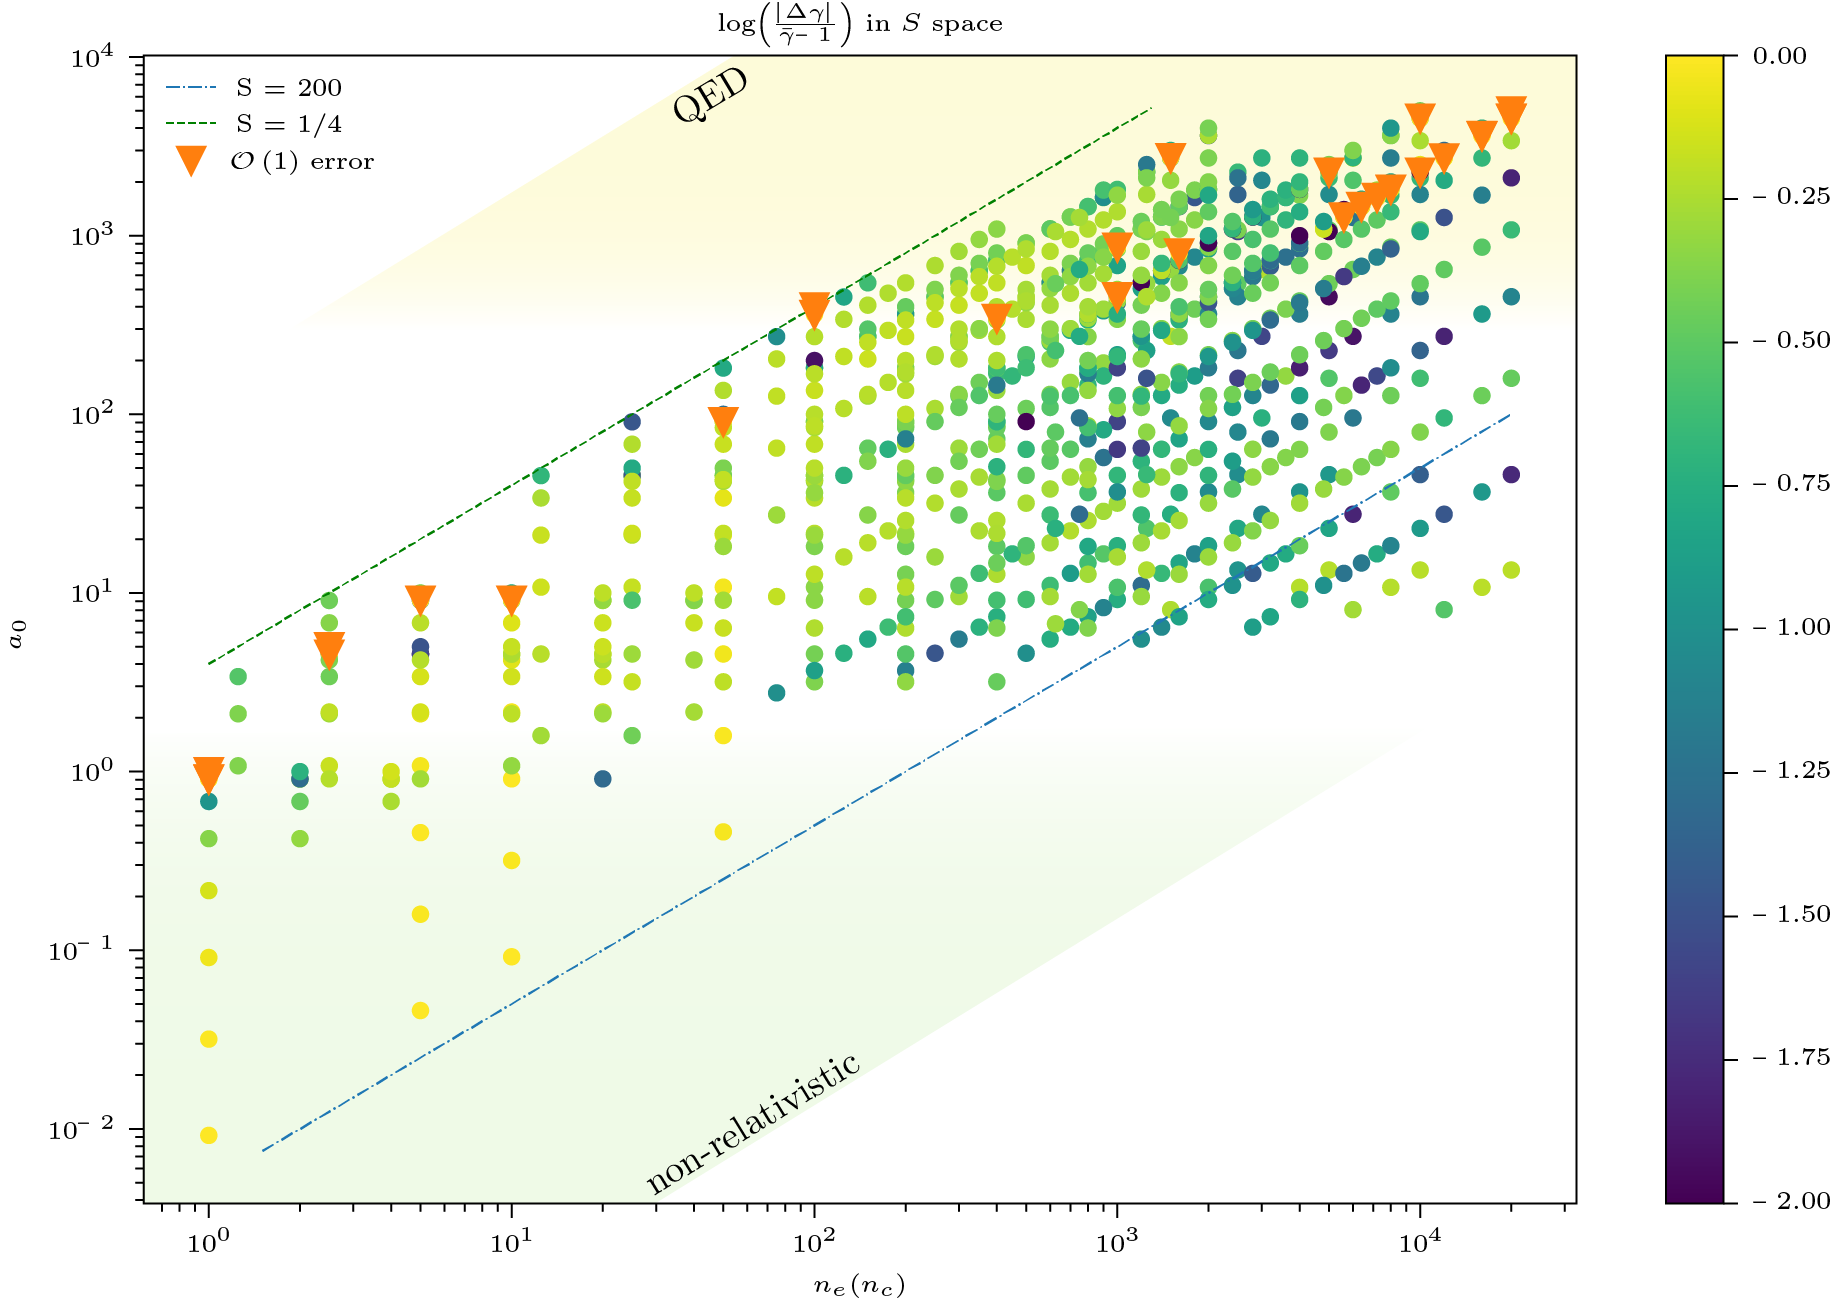
\includegraphics[width=1\linewidth]{figures/zvp/log_abs_error_T_edit}
	\caption[The relative errors for each mean energy data point compared to figure \ref{fig:zvpmeangammas}.]{The relative errors for each mean energy data point compared to figure \ref{fig:zvpmeangammas}. The orange triangles indicate data points for which the model fails to predict the mean energy.}
	\label{fig:zvp-logabserrortedit}
\end{figure}
Those points marked by an orange triangle have associated errors of over an order of magnitude. Reassuringly, such points occur only after the onset of QED effects, known to impact the ZVP mechanism \cite{savinEnergyAbsorptionLaserQED2019} and for $S<1$, that is, where the plasma becomes relativistically transparent to the laser pulse, a fundamentally different regime. Equally, for non-relativistic laser intensities, where assumptions of electron coherency cannot be made, are poorly fit by the model. It is particularly interesting that there is no indication that large $S$ causes a breakdown of the model, extending the applicability of the model further than previously considered and opening up the field to a wider range of conditions, such as that of shock compressed plasmas. To summarise, it would appear the ZVP model is valid for $10 \le a_0 \le 300$ and $S\ge1$.

\subsection{Energy absorption in the ZVP regime}\label{sec:zvp-energyabsorption}
As stated previously the laser-plasma coupling exists in a state of adiabaticity with the exception of the ZVP acceleration phase and hence equation \ref{eq:zvp_U} describes the absorption of laser pulse energy. For normal incidence, the rate of energy transfer is therefore
\begin{equation}\label{eq:zvp-rate}
	R = \frac{U\omega_\mathrm{L}}{\pi},
\end{equation}
since two bunches are produced per laser cycle. To demonstrate the scaling for $U$ in 2D PIC simulations, peak instantaneous electron bunch energies escaping to the rear of the bulk were extracted from those PIC simulations with $S=1$. For constant $S$, 
\begin{equation}
	U \sim a^2_0.
\end{equation}
Energies are plotted in figure \ref{fig:zvppeakgamma}.
\begin{figure}
	\centering
	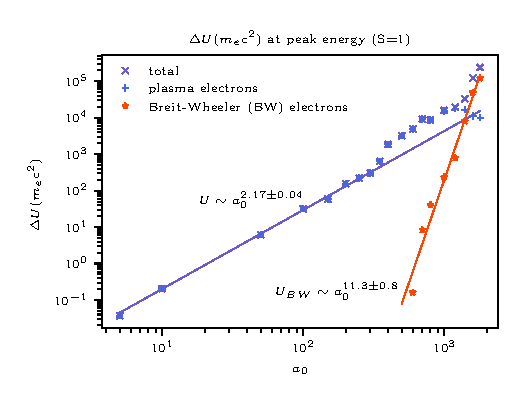
\includegraphics[width=0.7\linewidth]{figures/zvp/zvp_peak_gamma}
	\caption[Peak instantaneous bulk electron bunch total energy escaping to the plasma bulk rear.]{Peak instantaneous bulk electron bunch total energy escaping to the plasma bulk rear.}
	\label{fig:zvppeakgamma}
\end{figure}
Fitting the total energy within the range of validity established for the ZVP model finds
\begin{equation}
	U \sim a^{2.01\pm0.003}_0,
\end{equation}
reproducing with great success the anticipated scaling within the ZVP regime. It is also quite satisfying that the number of electrons and bunch mean energies both follow their anticipated ZVP scalings, further evidence this is not a simple ponderomotive effect. By extracting specific bunch total energies, rather than just the peak energies of the plasma block as a whole as was performed in previous studies, this is a far more direct confirmation of energy absorption by the ZVP mechanism into electron bunches. This is highlighted by the difference in results obtained for this study compared to a previous study by Savin \textit{et al} \cite{savinEnergyAbsorptionLaserQED2019} when investigating the QED regime as will be discussed later. It was not possible to reproduce the constants of equation \ref{eq:zvp_U} as the neutralising return current in the plasma bulk generates an electrostatic field on the rear side of the plasma block, decelerating bulk electron bunches as they escape the plasma. It should be possible to calculate the deceleration by considering the number of electrons expelled by the plasma. It is, however, clear from the simulations that at least some electrons in the escaping bunch are trapped by this rear-side potential well reducing its magnitude.

While equation \ref{eq:zvp_U} describes energy absorption into hot electron bunches, the coupling of such hot collisionless electrons to the bulk plasma given the lack of collisionality is naturally indirect. There are two key mechanisms \cite{sherlockIndepthPlasmawaveHeating2014}. Firstly, via a cooler resistive return current of electrons that neutralises the current of the injected hot electrons that escape the potential well of the front surface\textbf{ (cite this, the refernce in sherlock 2014 is not great)}. Since all hot electrons travel at approximately speed $c$, the magnitude of the return current depends not on the total energy absorbed but instead on the total number of electrons injected, as given by equation \ref{eq:zvp-Ne}, depending linearly on laser spot area and the electric field magnitude and not on the plasma density\footnote{Note that for a sufficiently thin target, the return current induces an electrostatic field on the back surface of the target which can then reflect hot electron bunches and decelerate them to the point of a return to collisionality. This is a reality for the PIC simulations explored in this thesis, however, since realistic targets are much thicker this shall be neglected.}. Secondly, via the formation of large amplitude bulk plasma waves induced in the wake of the hot electron bunches. Sherlock \textit{et al} \cite{sherlockIndepthPlasmawaveHeating2014} calculate the magnitude of the induced wakefield to be
\begin{equation}
	E_\mathrm{W} = \frac{eN_\mathrm{e}c}{\omega_\mathrm{p}\epsilon_0} = \sigma \sqrt{\frac{m_\mathrm{e}\epsilon_0}{n_\mathrm{e}}}E_\mathrm{L},
\end{equation}where here the bunch velocity has been set to $c$, bulk electrons will be accelerated by $E_\mathrm{W}$ and their kinetic energy converted to heat via collisions. Interestingly, this reproduces the mid temperature electon scaling with density that was observed by Chrisman \textit{et al} \cite{chrismanIntensityScalingHot2008} in their study of hot electron energy coupling in cone-guided fast ignition of inertial fusion targets. This is a different possible explanation to their self-declared `hand waving argument'. Excluding this study, such formulations for heat transfer to the plasma bulk within the ZVP regime remain untested in simulations.

Note also that as the laser pulse intensity rises, the fraction of energy absorbed by the ion species increases. Savin \cite{savinModellingLaserPlasmaInteractions2019} determined for $S=1/2$, $a_0 = 100$, that this would be almost 20\%. Energy is absorbed by ions via the hole boring mechanism as described elsewhere in this thesis.


\subsection{Unpacking the QED effects of figure \ref{fig:zvppeakgamma}}
In Savin's acclaimed paper \cite{savinEnergyAbsorptionLaserQED2019}, they determined theoretically and demonstrated in simulation that at $a_0 = 300$, $n_\mathrm{e} = 50 n_\mathrm{c}$, there is a transition from standard ZVP scalings to an enhanced QED scaling associated with \ac{BW} electrons increasing the pseudocapacitor plate charge. Explicitely,
\begin{equation}
	T \sim \frac{a^5_0}{\bar{n}_\mathrm{e}}.
\end{equation}
Such a scaling shift was not observed for the large parameter scan presented in figure \ref{fig:zvpmeangammas}. Simulations revealed this was likely due to only few \ac{BW} pairs being produced towards the plasma edges and hence no additional gain in energy from crossing the pseudocapacitor at those points. Another concern is Savin's study was conducted within the regime of relativistic transparency where it is unclear whether the ZVP potential well can be maintained and was not explored in this study. The final consideration is the well known effect of radiation trapping due to \ac{RR} \cite{jiRadiationReactionTrappingElectrons2014}, also observed in these PIC simulations. After acceleration across the pseudocapacitor, the electron bunch encounters the subsequent laser peak. If the electron bunch gamma factor and laser intensity are both large enough, electrons radiate a significant fraction of their energy and are thus stopped in their tracks. Unable now escape the potential well at the plasma surface they are trapped and are not observed to escape the plasma until the laser pulse intensity reduces. Such an effect would not impact Savin's scalings but would of course inhibit the observation of the scaling for electrons escaping to the sides and rear of the plasma block. Note that should this be the case and the collisionless electron bunches remain within the plasma bulk, Savin's ZVP QED model truly applies directly to energy absorption by the plasma bulk.

Returning now to figure \ref{fig:zvppeakgamma}, there are two interesting aspects. Firstly the sudden jump in total energy at $a_0 \approx$ 300. This cannot be explained by ZVP theory nor QED theory since the jump is observed with QED effects switched off. Secondly, the even sharper jump in total electron bunch energy above $a_0 = 1000$. Decomposing the total energy into bulk electrons (here refering to electrons from the plasma bulk that undergo ZVP) and those produced via the BW process, this is clearly a QED effect. Energy in BW produced electrons scales at a staggering
\begin{equation}
	U_\mathrm{BW} \sim a^{11.3\pm 0.8}_0,
\end{equation}
while the energy of bulk plasma electrons decreases. Perhaps this is a signal of Savin's QED ZVP electron bunches only at a higher energy due to the substantially greater plasma density of these simulations. The reduction in bulk electron energy can be attributed to an oversaturation of the front surface with BW electrons.

Combining equations \ref{eq:intro-photonchi} and \ref{eq:zvp_U} and assuming the electron radiates all its energy to the photon, for the ZVP mechanism, at the point of emission one finds
\begin{equation}
	\chi_\gamma =\frac{ \sqrt{2} |\mathbf{E}|}{E_\mathrm{S}}\frac{a^2_0}{\bar{n}_\mathrm{e}}.
\end{equation}
The probability of \ac{BW} pair production begins to rapidly increase around $\chi =1$, therefore, the transition to QED will occur at
\begin{equation}
	a_0 \approx \left(\frac{ E_\mathrm{S}}{\sqrt{2}}\frac{e\bar{n}_\mathrm{e}}{m_\mathrm{e}c\omega_\mathrm{L}}\right)^{1/3} = \left(\frac{a_\mathrm{s}\bar{n}_\mathrm{e}}{\sqrt{2}}\right)^{\frac{1}{3}},
\end{equation}
where $a_\mathrm{S} = \num{7.73e5}$ is the normalised vector potential associated with the Schwinger Field, thus explaining the transition to QED at higher intensities in this work compared to Savin's. Following Savin's theory, one expects
\begin{equation}
	U_\mathrm{QED} \sim \frac{a^7_0}{S},
\end{equation}
therefore much work is required to understand and unify these results, starting with the application of the methods of this analysis to the parameter space explored by Savin. Undoubtedly, the advent of next generation exa-watt scale lasers and access to this regime will be exceedingly interesting if such scalings in bunch energy can be maintained.

Linear Breit-Wheeler can safely be neglected, there is simply not enough energy in the system. For two interacting photons of energy $E_1$, $E_2$, by consideration of four-momenta, the threshold condition for pair production is 
\begin{equation}
	E_1E_2 \ge (m_\mathrm{e}c^2)^2.
\end{equation}
For a near-infrared laser photon of energy $\hbar \omega_\mathrm{L}$, the interacting photon must have an energy in excess of 200 GeV. Despite the extreme acceleration gradients considered in this thesis, the ZVP mechanism predicts photons of energies no greater than 10 GeV and thus linear Breit-Wheeler is suppressed.

He \textit{et al} \cite{heSinglelaserSchemeObservation2021} identified an alternative mechanism for linear \ac{BW} using solid density targets, where forwards- and back-scattered high energy radiation reaction produced photons interact within a hollowed out plasma channel. In the geometry of interest in this thesis, while photons are produced in both directions, their production is localised to the plasma surface and at no points do their paths cross and thus this mechanism does not occur.

% TODO: Explore transition regions, do MORE simulations to fill in the gaps.

% TODO To do: convergence of electron bunch energies with nppc and sim resolution.

\subsection{Errors}
To get some sense of the stability of the parameter scan, new simulations with tweaked parameters were created to explore the effects of including collisions, increasing the temperature to resolve the Debye length and particle merging. The results are presented in figure \ref{fig:zvperrorsources}. 
% TODO: Make this plot fraction errors instead
\begin{figure}
	\centering
	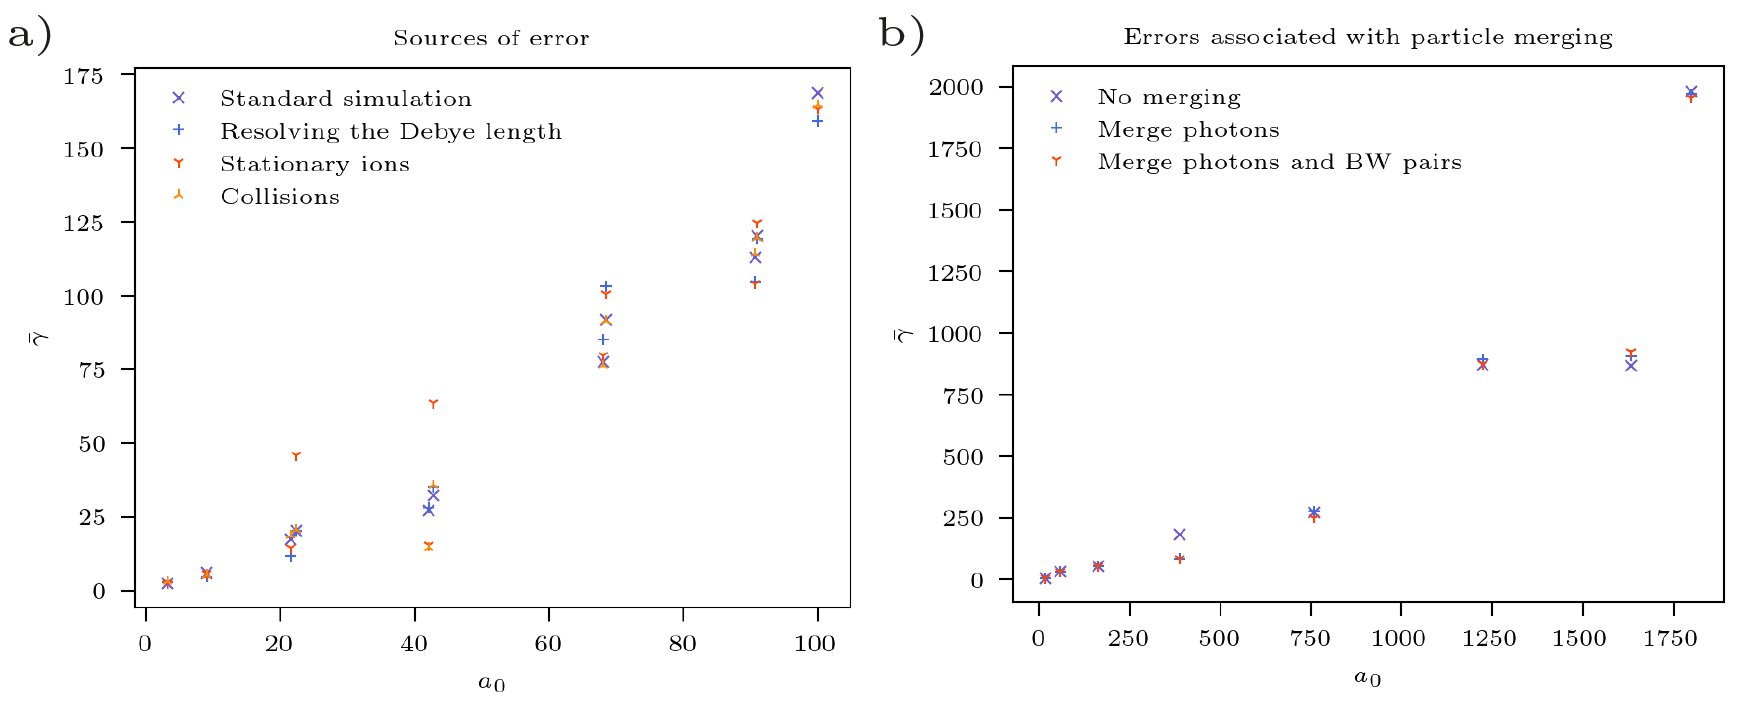
\includegraphics[width=1\linewidth]{figures/zvp/zvp_error_sources}
	\caption[An exploration of ZVP 2D PIC simulation stability.]{An exploration of ZVP 2D PIC simulation stability. a) Electron bunch mean energies extracted from simulations with $a_0$, $\bar{n}_\mathrm{e} =100$. Here, the $x$-axis is the normalised vector potential of the laser pulse cycle that made them, this is why there appears to be results stacked. b) Electron bunch mean energies extracted from simulations with $a_0$, $\bar{n}_\mathrm{e} =1800$ both with and without particle merging.}
	\label{fig:zvperrorsources}
\end{figure}
In general including collisions had little to no effect on the results and changing the Debye length had a small but not systematic effect on the results. Note that while numerical heating is not directly dependent on laser intensity, increases to $a_0$ would increase the electron bunch density. Thus, resolving the Debye length of the ultra-high density (orders of magnitude greater than solid density) electron bunches produced by the higher laser pulse intensities considered here is a non-trivial but potentially interestig exercise. Particle merging was essential for simulations with $a_0 > 1800$. At least at $a_0 = 1800$ it would appear particle merging had negligible impact, however it is likely the error would increase with $a_0$.

% TODO Next: finish QED discussion and QED section then do errors, then go through paper see if anything to add.

% TODO Also perhaps put in the plot of a laser of constant intensity and variation between bunches.

% TODO Also look again at fitting just to region where expression is valid.

\section{Planned future work}\label{sec:zvp-future_work}
Nothing is true unless it is measured and by now the reader should have a healthy level of skepticism for state-of-the-art PIC codes and their inherent proliferation of uncertainty. After a successful proposal application, four weeks of beam time have been awarded on the GEMINI-PW laser facility at the \ac{CLF} \cite{LaserSystemGemini}. Next July, the study of mass-limited ZVP electron bunches will be put to the test as part of a three-pronged experimental campaign, the main experimental goals are
\begin{enumerate}
	\item to characterise the X-ray \ac{HHG} emission from the reflection of a relativistic laser of a solid target, following on from a recent experiment at the ORION laser facility at AWE \cite{hoppsOverviewLaserSystems2013}, which is discussed in great detail in the following chapter;
	\item to simultaneously measure and correlate \ac{HHG} and the ZVP electron bunches responsible for the \ac{HHG} using a novel experimental setup;
	\item to apply the attosecond X-ray \ac{HHG} beam as a diagnostic tool in a proof of principle warm dense matter experiment.
\end{enumerate}
Preparations are now underway. The requirements for this experiment are simple: a relativistically intense high contrast laser pulse ($a_0 \ge 10$) of a few femtoseconds duration incident on a solid target with surface perturbations small compared to the wavelength of the laser pulse. A simulation describing the experimental setup for the ZVP bunch measurement is given in figure \ref{fig:experimentsetuphhgbunches2}. 
\begin{figure}
	\centering
	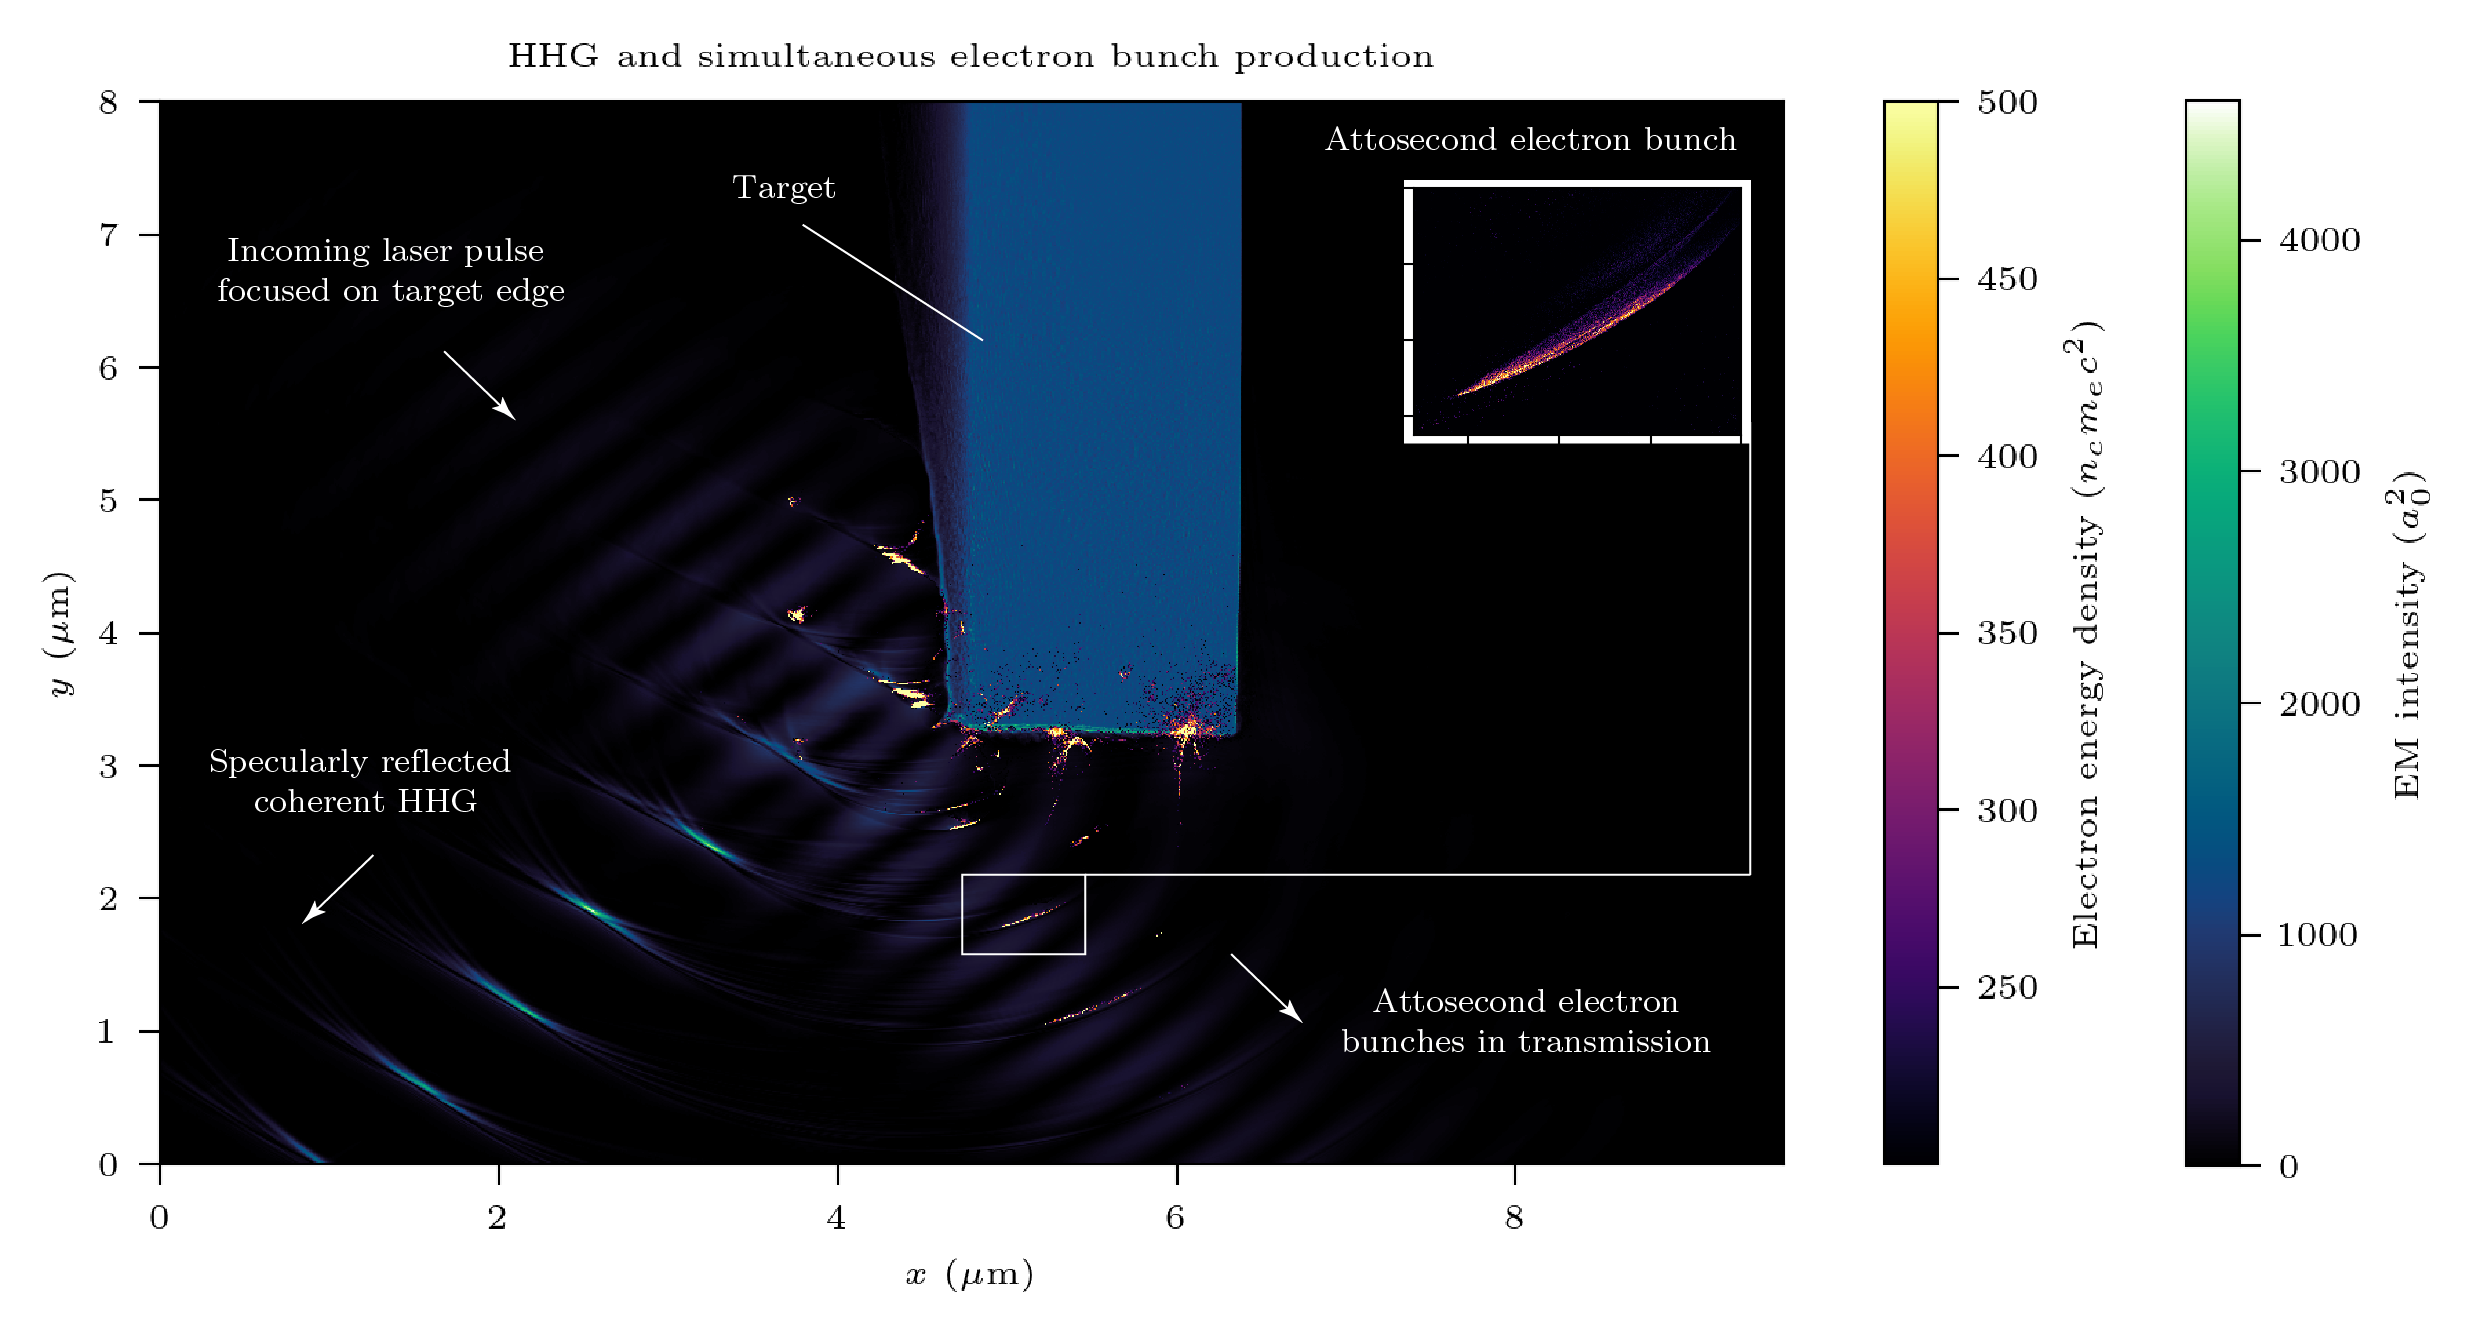
\includegraphics[width=1\linewidth]{figures/zvp/Experiment_setup_HHG_bunches2}
	\caption[Planned GEMINI-PW experimental setup for the measurement of ZVP electron bunches.]{A simulation of the planned GEMINI-PW experimental setup for the measurement of ZVP electron bunches. This novel setup enables the simultaneous measurement of attosecond ZVP electron bunches and their coherent emission of X-ray light. The GEMINI-PW laser pulse is incident at \qty{45}{\degree} on the low density polyethylene target with a preplasma scale length of $0.2\lambda_\mathrm{L}$. For this angle of incidence, transmitted bunches and specularly reflected X-ray harmonics are produced at a frequency of $\omega_\mathrm{L}$.}
	\label{fig:experimentsetuphhgbunches2}
\end{figure}
By focusing the laser onto the edge of a transversely mass-limited target, the emitted electron bunch energies will be maximised. Simulations suggest it should be possible to simultaneously measure the specularly reflected \ac{HHG} and the attosecond ZVP electron bunches that produce it. Directly linking the bunch qualities to the properties of the \ac{HHG}. Note via equations \ref{eq:zvp_N} and \ref{eq:zvp_T}, the low density target of Figure \ref{fig:experimentsetuphhgbunches2} will produce larger and more energetic bunches. They are therefore a more practical choice for the experiment relative to the aluminium targets of previous sections

Remaining actions include the performance of PIC code simulation parameter scans in the new geometry. While normal incidence was most convenient for these initial simulations, oblique incidence is more optimal for \ac{HHG} \cite{gonoskovUltrarelativisticNanoplasmonicsRoute2011, edwardsXRayEmissionEffectiveness2020} and as can be understood from equations \ref{eq:zvp_Tzvp_theta} and \ref{eq:zvp_Uzvp_theta}, the new energy scaling expressions for the ZVP mechanism at oblique incidence. Not only is oblique preferable but it is essential to mitigate damage to the laser optics via back-reflection. The \ac{HHG} beam intensity at focus can be over 1000 times that of the incident laser pulse \cite{quereReflectingPetawattLasers2021}. It is necessary, therefore, to test the new predictions for oblique incidence energy scalings and total electron bunch charge as well as the angle of bunch ejection, the non-zero transverse vector potential of the laser will prevent the bunch from propagating directly along the transmission axis. It would also be useful to perform a parameter scan of preplasma scale length. In this work so far, it was assumed that the optima for electron bunch production are simply those for \ac{HHG} given the intrinsic link between the two. \textbf{CITE THESE}. 

\subsubsection{GEMINI-PW laser facility}
The GEMINI-PW laser facility housed at the \ac{CLF} is a petawatt class facility consisting of two 30 fs beams each delivering a maximum focused intensity of \qty{2e21}{W.cm^{-2}} at a repetition rate of 0.05 Hz. Such high frequency of operation has led to a paradigm shift in high power laser physics experimentation with the arrival of statistically significant results.


\subsubsection{Targets}
A range of thick, flat solid targets are proposed to probe the density parameter space: diamond, a selection of plastics (polymethyl methacrylate, low and high density polyethylene and polycarbonate) and mirrored targets, which produced interesting and slightly unexpected results in the ORION experiment. It would also be interesting to produce foam targets gaining access the optimal low $S$ regime \cite{bataniPhysicsIssuesShock2014}. Target wheels will be used to take full advantage of the high shot rate of the GEMINI-PW laser. It is anticipated that due to focal spot jitter, not all shots will hit the target edges. 

\subsubsection{Diagnostics}
The electron bunches will be measured using an electron spectrometer placed a few centimetres from the target to measure the time-integrated energy spectrum. The spectrometer will be shielded from the laser pulse and any \ac{HHG} in transmission using a flash coated kapton foil which should not significantly hinder the MeV electron bunches produced in the interaction. Mordovanakis \textit{et al} used Image Plate stacks to obtain the electron bunch structure and emission angle, it may be necessary to perform this first to accurately position the spectrometer. While resolving attosecond durations remains an outstanding challenge of experimental science, it may be possible to measure the total duration of the train of attosecond electron bunches by measuring the characteristics of coherent optical transition radiation produced by the electrons upon incidence on a secondary target \cite{linIsolatedAttosecondElectron2020}. The X-ray \ac{HHG} emission will be measured using the OHREX spectrometer \cite{beiersdorferLineshapeSpectroscopyVery2016} on loan from ORION, a spherically bent crystal spectrometer with ultra-high resolution and high-signal-to-noise ratio. Lower order harmonics will be measured using angularly resolved EUV spectrometers. Note that in the absence of attosecond resolution diagnostics, measuring the harmonic spectrum of the coherent \ac{HHG} is the only way to reconstruct the temporal shape of the pulse. Simulations have suggested that the reflected spectrum produced by Coherent Synchrotron Emission of the electron bunches is approximately Fourier-limited \cite{cousensElectronTrajectoriesAssociated2020}. Off-axis spectrometers should be used to compare the signals to the background emission and to measure the plasma temperature \cite{akliDualChannelXray2010}. A quarter wave plate could be used to convert the incoming laser pulse to a circular polarisation to compare the signals to those detected in the absence of zeros in the vector potential.

\subsubsection{Preplasma scale lengths and prepulse control}
Observation of the ZVP mechanism requires a sufficiently steep density gradients at the laser-plasma interface. A potential drawback of \ac{CPA} laser systems is the existence of prepulses that heat targets, causing them to expand significantly before arrival of the main pulse. To increase the laser contrast, to the point where there is no preplasma formation, GEMINI-PW utilises a Double Plasma Mirror setup \cite{doumyCompleteCharacterizationPlasma2004}. Each mirror is an anti-reflection coated optic placed in the path of the laser beam, acting as an optical switch. As the laser fluence passes the damage threshold of the optic, plasma forms on the front surface and the mirror starts to reflect. As it has been suggested that there is an optimum scale length for \ac{HHG}, the second GEMINI-PW beam will be used to generate a controllable prepulse to tailor the plasma surface. Investigation of preplasma generation will occur in parallel to the main experimental goals.

\section{Conclusions}\label{sec:zvp-conclusion}
% TODO: 3D3V mention somewhere
The Zero Vector Potential mechanism describes the post-ponderomotive rapid absorption of ultra-relativistic laser energy by a solid density overdense, collisionless and fully ionised plasma on the timescales of ion immobility. The defining characteristics of the mechanism have been identified in 3D PIC simulations including the observation of a zero of the vector potential propagating at speed $\approx 1.4c$ through a high density ZVP electron bunch at the front surface of the plasma early in ablative journey of the electron bunch. Simulations have suggested that from currently operating 10 PW short pulse laser facilities and foam targets, the ZVP mechanism can produce a train of attosecond duration, nano-Coulomb electron bunches, each with a transverse emittance of a few $\unit{nm.rad}$. Such charge and quality is comparable to state-of-the-art electron bunch accerators but on paradigm shifting timescales. Such timescales being those on which atomic processes occur, these electron bunches could be manipulated to literally `shed light' onto fundamental biological and chemical processes. Via a massive 2D PIC parameter scan the energies of such mass-limited electron bunches have been compared to those predicted by the ZVP model, identifying a range of validity for the model, specifically $a_0>10$, $S>1$. These simulations were also used to confirm the energy absorption scaling in 2D up to and into the QED regime. Finally, details were provided on the planned GEMINI-PW experiment where ZVP electron bunches and ZVP absorption could be observed for the first time. Taking a slight rollback in laser power, the following chapter will now switch gears from absorption to the reflection of radiation from a solid target in the discussion of a recent experiment at the moderately relativistic ORION laser facility.